\documentclass[a4paper, 12pt]{article}
\usepackage[a4paper, total={6in, 8in}]{geometry}
\geometry{
	a4paper,
	left = 1.5 cm,
	right = 1.5 cm,
	top = 2cm,
	bottom = 2.5 cm,
}
\usepackage[T1]{fontenc}
\usepackage{pythontex}
\usepackage{hhline}
\usepackage{array,booktabs}
\newcolumntype{M}[1]{>{\centering\arraybackslash}m{#1}}
\usepackage[table]{xcolor}
\usepackage{caption}
\usepackage{makecell}
\usepackage{lipsum}
\usepackage{pifont}
\usepackage{amssymb}
\usepackage{amsmath}
\usepackage[utf8]{inputenc}
\usepackage[italian]{babel}
\usepackage{graphicx}
\graphicspath{ {./images/} }
\usepackage{spverbatim}
\usepackage{float}
\usepackage{url}
\usepackage{xstring}
\usepackage{hyperref}
\usepackage{xcolor}
\usepackage{upquote}
\definecolor{linkcolor}{RGB}{1,1,87}
\hypersetup{
    colorlinks,
    citecolor=black,
    filecolor=black,
    linkcolor=linkcolor,
    urlcolor=blue
}
\usepackage{fancyvrb,newverbs,xcolor}
\definecolor{cverbbg}{gray}{0.93}
\definecolor{cellcolor}{RGB}{165,194, 242}
\usepackage{xifthen}
\usepackage{multirow}
\usepackage{adjustbox}
\usepackage{listings}
\lstset{
  basicstyle=\ttfamily,
  backgroundcolor=\color{cverbbg},
  breaklines=true,
  frame=lines,
  framerule=1pt,
  numbers=left,
  numbersep=10pt, 
  keywordstyle=\color{blue},
  commentstyle=\color{green!60!black},
  stringstyle=\color{red},
  showstringspaces=false,  
  framextopmargin=1.5ex,
  framexbottommargin=1.5ex,
  framexleftmargin={\dimexpr 1.5em+3pt},
  xleftmargin={\dimexpr 1.5em+3pt},
  linewidth={\dimexpr \linewidth-3pt},
}

% following restart section enumeration in different \part
\usepackage{chngcntr}
\counterwithin*{section}{part}

\newcommand{\makesub}[1]{%
  \saveexpandmode\noexpandarg
  \StrSubstitute{#1}{\_}{_}[\temp]%
  \restoreexpandmode%
}

\newcommand{\target}[1]{%
  \makesub{#1}%
  \hypertarget{\temp}{}%
}

\newcommand{\attach}[1]{%
  \makesub{#1}%
  \hyperlink{\temp}{\emph{#1}}%
}
\newcommand{\attachcode}[1]{%
  \makesub{#1}%
  \hyperlink{\temp}{\code{#1}}%
}

\newcommand{\code}[1]{\colorbox{cverbbg}{	exttt{\detokenize{#1}}}}
%\newcommand{\code}[1]{\colorbox{cverbbg}{\texttt{\StrSubstitute{#1}{_}{\_}}}}

\newcommand{\linux}{\textit{Linux}}
\newcommand{\win}{\textit{Windows}}
\newcommand{\nota}[1]{\textbf{Nota}: #1}
\newcommand{\memo}[1]{\textbf{Memo}: #1}
\newcommand{\esempio}[1]{\textbf{Esempio}: #1}
\newcommand{\tbs}{\textbackslash}
\newcommand{\Null}{\code{NULL}}
\newcommand{\api}{\emph{API}}
\newcommand{\key}[1]{\texttt{\StrSubstitute{#1}{_}{\_}}}
\usepackage{eurosym}

\newcommand{\paramtable}[2][]{%
\ifthenelse{\isempty{#2}} {\input{|"/home/luca/latex_scripts/generate_param_table.py '#1'"}} {\input{|"/home/luca/Scrivania/MA/homeworks/homework-04/report/scripts/generate_param_table.py '#1' '#2'"}}%
}

\newcommand{\hr}[0]{\begin{center}%
\line(1,0){450}%
\end{center}%
}

\newcommand{\xmark}[0]{\ding{55}}
\newcommand{\vmark}[0]{$\checkmark$}

\newenvironment{myverb}
 {\SaveVerbatim{cverb}}
 {\endSaveVerbatim
  \flushleft\fboxrule=0pt\fboxsep=.5em
  \colorbox{cverbbg}{%
    \makebox[\dimexpr\linewidth-2\fboxsep][l]{\BUseVerbatim{cverb}}%
  }
  \endflushleft
}

\setcounter{tocdepth}{4}
\setcounter{secnumdepth}{4}
\setlength\parindent{0pt}
\newcommand{\image}[1]{\input{|"/home/luca/latex_scripts/add_image.py '#1'"}}

%%%%%%%%%%%%%%%%%%%%%
\newcommand{\bup}[0]{$\mathcal{B} \cup \mathcal{P}$}


\begin{document}

\title{
    \textbf{    
        \emph{Simulazione PMCSN}
    }
}
\author{Luca Mastrobattista, 0292461}
\date{} %no date wanted
\maketitle  



\tableofcontents

\newpage
\section{Traccia della Simulazione}
\subsection{Caso di studio}
Si vuole valutare l'opportunità di aprire un locale in un piccolo paese che offrirà servizi di bar e pizzeria. Il locale è già dotato di tutto l'arredamento e verrà affittato al costo mensile di 1.500,00 $\mbox{\euro}$. Il pizzaiolo selezionato per il servizio di pizzeria ha indicato che nel forno disponibile è possibile preparare contemporaneamente un massimo di 2 pizze, ciascuna delle quali richiede in media 3 minuti di preparazione. Inoltre, è stato concordato con il pizzaiolo che lavorerà tutti i giorni della settimana dalle 19:00 alle 23:00, con una retribuzione giornaliera di 50 euro, con l'accordo che tutte le ordinazioni ricevute prima delle 23:00 verranno comunque servite, anche se ciò richiederà di continuare a cuocere pizze oltre quell'orario. Per quanto riguarda le richieste relative al bar, si desidera che "l'ultimo giro" venga chiamato alle 02:00, senza accettare ulteriori richieste dopo quell'orario, ma completando tutte quelle già presenti.\\

Dopo un'osservazione settimanale di altri locali che offrono servizi simili, è emerso che il numero di clienti che frequentano il locale varia nelle diverse fasce orarie della giornata. Inoltre, durante il fine settimana, si registra un aumento della frequenza delle richieste rispetto ai giorni feriali. Infine, è stato notato che nella fascia oraria compresa tra le 15:00 e le 18:00 le richieste sono così scarse che non è conveniente mantenere il locale aperto. Di seguito sono riportate delle tabelle riassuntive per le frequenze di arrivo.

\target{tabelle riassuntive dei tassi di arrivo}
\begin{table}[!htb]
\begin{minipage}{.5\linewidth}
\centering
    
\begin{tabular}{ |c|c|c| }
\hline
\cellcolor{cellcolor}Fascia oraria & \cellcolor{cellcolor}$\lambda${\textsubscript{B,W}} & \cellcolor{cellcolor}$\lambda${\textsubscript{P,W}} \\
	\hline
	\hline
    07:00 $\rightarrow$ 11:00 & 30 j/h & \xmark \\
    \hline
    11:00 $\rightarrow$ 15:00 & 12.5 j/h & \xmark \\
    \hline
    15:00 $\rightarrow$ 18:00 & \xmark & \xmark \\
    \hline
    18:00 $\rightarrow$ 19:00 & 25 j/h & \xmark \\
    \hline
    19:00 $\rightarrow$ 23:00 & 12.5 j/h & 10 j/h \\
    \hline
    23:00 $\rightarrow$ 02:00 & 10 j/h & \xmark \\
    \hline
    \end{tabular}
	\bigskip 
	       
	\textit{Frequenze di arrivo settimanali} 
\end{minipage}
\begin{minipage}{.5\linewidth}
\centering
\begin{tabular}{ |c|c|c| }
\hline
\cellcolor{cellcolor}Fascia oraria & \cellcolor{cellcolor} $\lambda${\textsubscript{B,WE}} & \cellcolor{cellcolor}$\lambda${\textsubscript{P,WE}} \\
	\hline
	\hline
	07:00 $\rightarrow$ 13:00 & 30 j/h & \xmark \\
	\hline
	13:00 $\rightarrow$ 18:00 & 20 j/h & \xmark \\
    \hline
	15:00 $\rightarrow$ 18:00 & \xmark & \xmark \\
    \hline
    18:00 $\rightarrow$ 19:00 & 45 j/h & \xmark \\
    \hline
    19:00 $\rightarrow$ 23:00 & 22.5 j/h & 30 j/h \\
    \hline
    23:00 $\rightarrow$ 02:00 & 20 j/h & \xmark \\
    \hline
    \end{tabular}
	\bigskip 
	   
	\textit{Frequenze di arrivo fine-settimanali} 
\end{minipage} 
\end{table}

\bigskip

\subsection{Obiettivi}
L'obiettivo dell'analisi è determinare il numero ottimale di baristi da assumere per massimizzare i guadagni, tenendo conto di alcune condizioni e vincoli specifici.\\

Si considera una retribuzione di 40,00 $\mbox{\euro}$ al giorno per ciascun barista, con un turno lavorativo di 8 ore. Si presume che ogni barista sia in grado di servire un'ordinazione in 2 minuti, durante i quali si dedica esclusivamente a quella richiesta. Si assume inoltre che il prezzo medio delle richieste al bar sia di 5,00 $\mbox{\euro}$, mentre quello delle richieste alla pizzeria sia di 10,00 $\mbox{\euro}$. Tuttavia, esistono alcuni vincoli che si vuole che siano sempre rispettati:
\begin{itemize}
\item Ogni ordinazione al bar deve essere servita entro un massimo di 3 minuti.
\item Ogni ordinazione per la pizzeria deve essere servita entro un massimo di 10 minuti.
\end{itemize}

Per massimizzare i guadagni, è necessario determinare quanti baristi assumere in modo che siano sufficienti a gestire il flusso di ordini, mantenendo comunque i tempi di servizio entro i limiti stabiliti dai vincoli; inoltre, per rispettare i vincoli, si può valutare l'assunzione di un nuovo pizzaiolo e l'acquisto di un forno più grande.

\section{Modello concettuale}
\subsection{Visualizzazione grafica}
\begin{figure}[H]
\centering
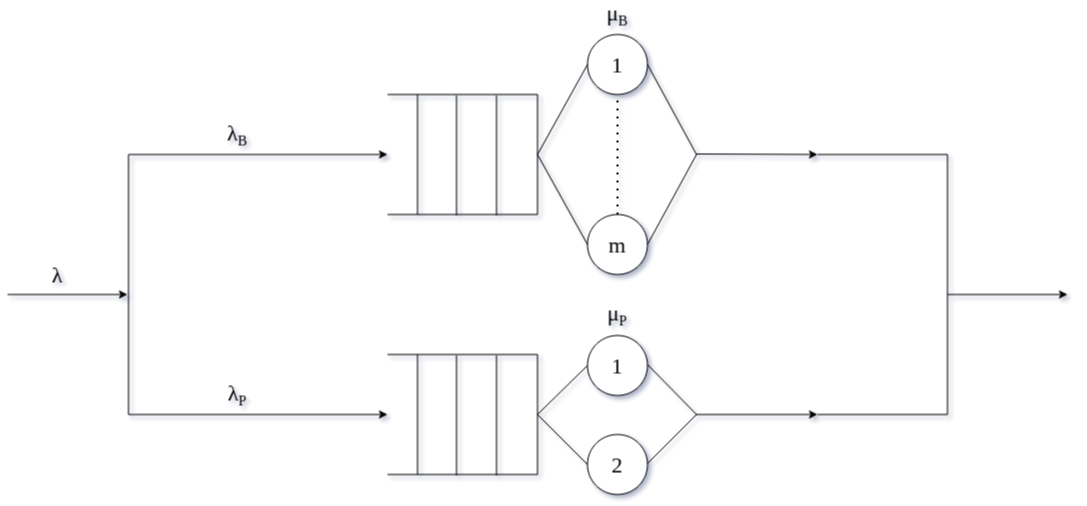
\includegraphics[width=\textwidth]{conceptual_model}
\end{figure}

La frequenza di arrivo $\lambda$ si compone della frequenza di arrivo $\lambda_B$ e $\lambda_P$, che sono rispettivamente i tassi di arrivo per richieste al bar e alla pizzeria. Una opportuna coda per ogni tipologia rappresenta la lista di attesa della tipologia stessa. Ogni servente di tipo \textit{B} rappresenta un barista assunto, che lavora con una frequenza $\mu_B$. Ogni servente di tipo \textit{P}, invece, rappresenta una delle due richieste che il pizzaiolo è in grado di gestire contemporaneamente e lavora con frequenza $\mu_P$.


\subsection{Eventi del sistema e variabili di stato}
\subsection{Eventi}
\begin{center}

\begin{tabular}{ |c|c|c|c| }
	\hline
    \cellcolor{cellcolor}Indice & \cellcolor{cellcolor}Descrizione & \cellcolor{cellcolor}Attributo 1 & \cellcolor{cellcolor}Attributo 2 \\
    \hline
    \hline
    0 & Arrivo di tipo B & t & x \\
    \hline
    1 & Completamento dal server $B_1$ & t & x \\
    \hline
    .. & .. & t & x \\
    \hline
    m & Completamento dal server $B_m$ & t & x \\
    \hline
    m + 1 & Arrivo di tipo P & t & x \\
    \hline
    m + 2 & Completamento dal server $P_1$ & t & x \\
    \hline
    m + 3 & Completamento dal server $P_2$ & t & x \\
    \hline
    m + 4 & Evento di campionamento & t & x \\
    \hline
\end{tabular}
\end{center}
L'attributo \key{t} indentifica il tempo schedulato per la successiva occorrenza dell'evento di quel tipo; l'attributo \key{x} identifica lo stato di attività
dell'evento.

\subsection{Variabili di stato}
\begin{itemize}
  \item $l\textsubscript{B}(t)$: numero di richieste di tipo B al centro all'istante $t$
  \item $l\textsubscript{P}(t)$: numero di richieste di tipo P al centro all'istante $t$
  \item $X\textsubscript{s}(t)$: stato del servente $s$ all'istante $t$, 
  con $s \in$ \bup, dove \bup{} è l'insieme dei serventi di tipo \textit{B} unito all'insieme dei serventi di tipo \textit{P}.
  \[
      X\textsubscript{s}(t) = 
  \begin{cases}
      1& \text{se servente s è occupato}\\ 
      0              & \text{altrimenti}
  \end{cases}
  \]	
\end{itemize}

\section{Modello delle specifiche}

\subsection{Periodo di osservazione}
Il periodo di osservazione copre una giornata lavorativa composta dalle fasce orarie precedentemente riportate nelle \attach{tabelle riassuntive dei tassi di arrivo}. Questa giornata lavorativa può essere considerata sia durante la settimana (\textit{week}) che nel fine settimana (\textit{weekend}): è importante valutare il sistema in entrambi i casi poiché il flusso di richieste in ingresso varia tra i giorni lavorativi e i giorni feriali.

%Il periodo di osservazione è quello di un giorno lavorativo composto dalle due fasce orarie riportate precedentemente nelle \attach{tabelle riassuntiva dei tassi di arrivo}. Il giorno lavorativo può essere settimanale o feriale (\textit{week} è \textit{weekend}), ed è opportuno valutare il sistema in entrambi i casi a causa della variazione del flusso delle richieste in ingresso.

\target{interarrivi gaussiani}
\subsection{Distribuzione degli arrivi}
I valori dei tassi di arrivo sono stati raccolti attraverso l'analisi di dati reali, fornendo una stima attendibile ma flessibile. Per modellare il processo degli arrivi, è stata scelta la distribuzione esponenziale, con un tasso di arrivo $\lambda$ variabile per ciascuna fascia oraria. Tuttavia, per catturare le variazioni nei tempi di arrivo dei clienti, si è introdotto un elemento di realismo attraverso l'utilizzo di una distribuzione gaussiana all'interno di ciascuna fascia oraria. Questa scelta è basata sulle seguenti motivazioni:
\begin{itemize}
\item Flessibilità del modello: L'utilizzo della distribuzione esponenziale come base del modello offre una notevole flessibilità, consentendo la generazione di tempi di interarrivo casuali che possono variare significativamente. Questa flessibilità riflette in modo accurato la natura casuale degli arrivi in un bar, che può manifestare variazioni significative nel tempo, anche quando la frequenza di arrivo media è nota.

\item Introduzione del ritardo gaussiano: L'introduzione di un ritardo gaussiano arricchisce ulteriormente il modello, consentendo di tenere conto di effetti come le ore di punta o i momenti in cui ci si aspetta una maggiore affluenza. Questo approccio rende il modello più aderente alla realtà senza la necessità di creare un modello basato completamente su una distribuzione gaussiana, che potrebbe non rappresentare in modo accurato la variabilità dei tempi di interarrivo.
\end{itemize}



%Per modellare questo, si definiscono delle frequenze di interarrivo medie per ogni fascia oraria, riportate qui in minuti:
%\bigskip

%\begin{minipage}{.5\textwidth}
%\centering             
%\begin{tabular}{ |c|c|c| }
%	\hline
%    \cellcolor{cellcolor} Fascia oraria & \cellcolor{cellcolor}$\lambda${\textsubscript{B,W}} & \cellcolor{cellcolor}$\lambda${\textsubscript{P,W}} \\
%	\hline
%    \hline
%
%	07:00 $\rightarrow$ 11:00 & 0.5 j/min & \xmark \\
%
%    \hline
%    
%
%	11:00 $\rightarrow$ 15:00 & 0.21 j/min & \xmark \\
%
%    \hline
%    
%
%	18:00 $\rightarrow$ 19:00 & 0.42 j/min & \xmark \\
%
%    \hline
%    
%
%	19:00 $\rightarrow$ 23:00 & 0.21 j/min & 0.17 j/min \\
%
%    \hline
%    
%
%	23:00 $\rightarrow$ 02:00 & 0.17 j/min & \xmark \\
%
%    \hline
%\end{tabular}
%\bigskip
%              
%\textit{Frequenze di arrivo settimanali}
%\end{minipage}
%%
%\begin{minipage}{.5\textwidth}
%\centering
%\begin{tabular}{ |c|c|c| }
%	\hline
%    \cellcolor{cellcolor}Fascia oraria & \cellcolor{cellcolor}$\lambda${\textsubscript{B,WE}}
%    &\cellcolor{cellcolor} $\lambda${\textsubscript{P,WE}} \\
%    \hline
%    \hline
%	07:00 $\rightarrow$ 11:00 & 0.5 j/min & \xmark \\ 
%    \hline
%	11:00 $\rightarrow$ 15:00 & 0.34 j/min & \xmark \\
%    \hline
%	18:00 $\rightarrow$ 19:00 & 0.75 j/min & \xmark \\
%    \hline
%	19:00 $\rightarrow$ 23:00 & 0.375 j/min & 0.5 j/min \\
%    \hline
%	23:00 $\rightarrow$ 02:00 & 0.34 j/min & \xmark \\
%    \hline
%\end{tabular}
%\bigskip
%              
%\textit{Frequenze di arrivo fine-settimanali} 
%\end{minipage} 
%\bigskip

Per ogni fascia oraria si definisce una distribuzione di probabilità gaussiana:\\

\begin{minipage}{0.45\textwidth}
\begin{table}[H]
\centering
\begin{tabular}{ |c|c|c|c| }
	\hline
    \cellcolor{cellcolor} Fascia oraria & \cellcolor{cellcolor}$\mu$ & \cellcolor{cellcolor}$\sigma$ & \cellcolor{cellcolor}Link all'immagine\\
	\hline
    \hline

  	07:00 $\rightarrow$ 11:00 & 8 & 1.2 & \hyperlink{distribuzione gaussiana 7-11}{Link}\\
    \hline	
	
	11:00 $\rightarrow$ 15:00 & 13.5 & 2 & \hyperlink{distribuzione gaussiana 11-15}{Link}\\
    \hline
  
	18:00 $\rightarrow$ 19:00 & 18.5 & 0.4 & \hyperlink{distribuzione gaussiana 18-19}{Link}\\   
    \hline
    
	19:00 $\rightarrow$ 23:00 & 22.5 & 2 & \hyperlink{distribuzione gaussiana 19-23}{Link}\\
    \hline
    
    23:00 $\rightarrow$ 02:00 & 24 & 0.9 & \hyperlink{distribuzione gaussiana 23-26}{Link}\\ 
    \hline        
\end{tabular}
\end{table}
\end{minipage}
\hspace{0.1\textwidth}
\begin{minipage}{0.45\textwidth}
\begin{table}[H]
\centering
\begin{tabular}{ |c|c|c|c| }
	\hline
    \cellcolor{cellcolor} Fascia oraria & \cellcolor{cellcolor}$\mu$ & \cellcolor{cellcolor}$\sigma$ & \cellcolor{cellcolor}Link all'immagine\\
	\hline
    \hline
    19:00 $\rightarrow$ 23:00 & 20.5 & 1 & \hyperlink{distribuzione gaussiana P}{Link}\\
    \hline
\end{tabular}
\end{table}
\end{minipage}
\bigskip

\begin{minipage}{0.45\textwidth}
\centering
\textit{Parametri delle gaussiane per richieste di tipo B}
\end{minipage}
\hspace{0.1\textwidth}
\begin{minipage}{0.45\textwidth}
\centering
\textit{Parametri delle gaussiane per richieste di tipo P}
\end{minipage}
\bigskip

Per comprendere meglio come funziona il calcolo dei tempi di interarrivo, esaminiamo un esempio specifico. Per esempio, supponiamo di essere all'istante di simulazione $t_0$ di un giorno lavorativo settimanale, all'interno della prima fascia oraria, dove $\lambda$ è pari a 0.5 arrivi al minuto. Per calcolare il prossimo tempo di interarrivo, utilizziamo la seguente formula:
\[
	\frac{\texttt{Exponential(1/}\lambda)}{f^n(t_0)}
\]
Dove $f^n(t_0)$ rappresenta il valore della distribuzione di probabilità gaussiana relativa alla fascia oraria valutata in $t_0$, troncata riespetto all'intera fascia oraria. Nel nostro esempio specifico:
\[
	f^n(t_0) = \frac{f(t_0)}{F(11) - F(7)}
\]
dove $F(x)$ funzione cumulativa della distribuzione gaussiana relativa alla fascia oraria dalle 07:00 alle 11:00.\\

È importante sottolineare che non è stata adottata direttamente una distribuzione gaussiana per i tempi di interarrivo perché questa avrebbe modellato un comportamento diverso, dove i tempi sarebbero concentrati intorno al valore medio della distribuzione per l'intera fascia oraria. L'obiettivo era invece modellare una diminuzione dei tempi di interarrivo in prossimità di determinati momenti. È tuttavia possibile disabilitare questa opzione di ritardo gaussiano durante la simulazione tramite l'apposito flag a riga comando, conferendo al simulatore la flessibilità di adattarsi alle diverse esigenze di modellazione.

\subsection{Assunzioni}
\begin{itemize}
  \item Stato iniziale vuoto: 
  \[ 
    l\textsubscript{B}(0) + l\textsubscript{P}(0) = P(0) + B(0) = 0 
\]
  Come conseguenza, il primo evento deve essere necessariamente un arrivo e, in particolare, è un arrivo di tipo \textit{B}: la pizzeria apre alle 19.
  \item Stato finale di ogni giorno vuoto:
\[
    X\textsubscript{s}(T) = 0\ \ \ \forall s \in \mathcal{B} \cup \mathcal{P}
\]
  Con $T$ tempo di chiusura giornaliero e $\mathcal{B} \cup \mathcal{P}$ l'unione dell'insieme dei serventi di tipo \textit{B} e \textit{P}. Come conseguenza, l'ultimo evento non può essere un arrivo, e sarà quindi o una partenza o un campionamento.

  \item I tempi di servizio di ognuno dei serventi si assumono  esponenziali e indipendenti dalla fascia oraria. In particolare, ogni servente di tipo \textit{B} lavora con frequenza media pari a $\mu\textsubscript{B} = \frac{1}{2}\ j/min$; ogni servente di tipo \textit{P} lavora con frequenza media pari a $\mu\textsubscript{P} = \frac{1}{3}\ j/min$. 
  
\item l'evento di campionamento non deve seguire un evento di campionamento: non ha molto senso raccogliere due volte le statistiche se nel mezzo non è accaduto niente. Anzi: un campionamento incontrollato di questo tipo darebbe un peso maggiore al valore delle statistiche raccolte successivamente.
\end{itemize}

\subsection{Guadagni e costi}


\section{Modello analitico}
Di seguito sono riportaet le formule utilizzate per l’analisi teorica del sistema. In particolare, tutti i centri sono stati modellati come M/M/m per i quali si hanno le seguenti formule teoriche:
\begin{minipage}{0.5\textwidth}
\begin{itemize}
\item[] \[
P(0) = \left[\sum_{i=0}^{m-1} \frac{(m\rho)^i}{i!} + \frac{(m\rho)^m}{m!(1-\rho)}\right]^{-1}
\]
\item[] \[
P_Q = \frac{(m\rho)^m}{m!(1-\rho)} \cdot p(0)
\]

\item[] \[
E(TQ) = \frac{P_Q E(S)}{1-\rho}
\]
\end{itemize}
\end{minipage}
\begin{minipage}{0.5\textwidth}
\begin{itemize}
\item[] \[
E(TS) = E(TQ) + E(S_i)
\]
\item[] \[
E(NQ)_{Erlang} = \frac{PQ \rho}{1-\rho}
\]

\item[] \[
E(NS) = E(NQ) + m\rho
\]
\end{itemize}
\end{minipage}



\section{Modello computazionale}
Il modello computazionale è stato sviluppato in linguaggio \textit{Python} ed è implementato nel programma \texttt{simulation.py}. All'interno della cartella \key{configuration/}, sono conservati tutti i file di configurazione utilizzati nel corso dell'analisi, e questo è anche il percorso in cui vengono salvati eventuali nuovi file di configurazione. I parametri configurabili e i loro valori di default sono definiti nel file \key{configurations/Config.py}. \\

Il programma può essere eseguito da riga di comando, e offre diversi flag che ne influenzano il comportamento. È possibile ottenere un elenco di questi flag eseguendo il comando \key{python simulation.py -h} o \key{python simulation.py --help}, il quale restituirà il seguente messaggio:
\begin{figure}[H]
\centering
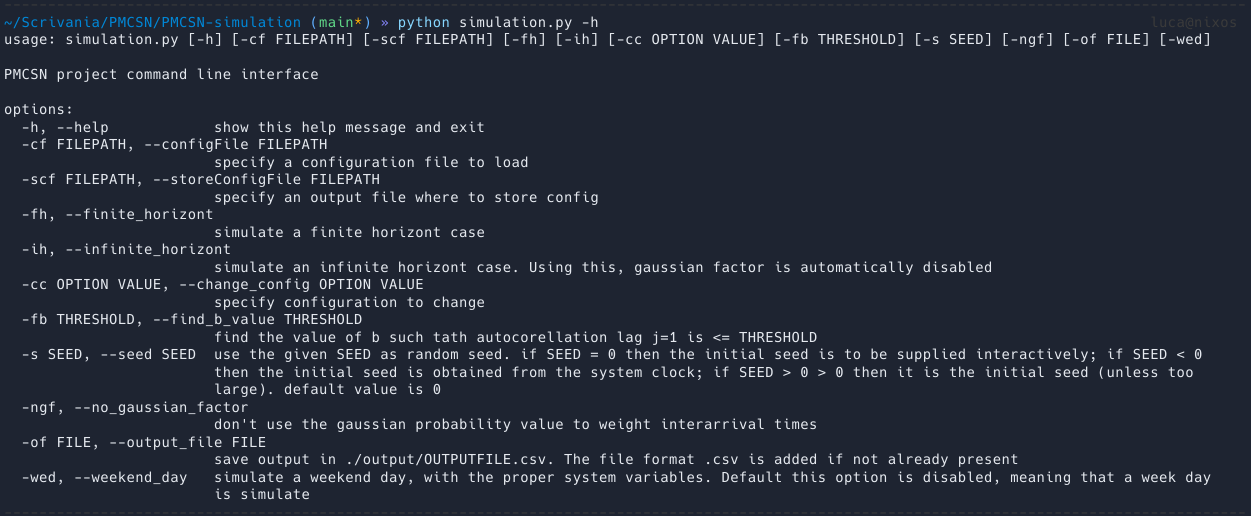
\includegraphics[width=0.8\textwidth]{program_help}
\end{figure}

Tra questi, il flag \key{-cc} consente di modificare qualsiasi impostazione presente nel file di configurazione specificando il valore desiderato direttamente da riga di comando, mentre il flag \key{-ngf}, ovvero \key{--no_gaussian_factor}, disabilita la normalizzazione del tempo di interarrivo utilizzando il fattore gaussiano determinato secondo le modalità descritte nella \hyperlink{interarrivi gaussiani}{sezione dedicata alla distribuzione degli arrivi}. \\.

%In particolare, col flag \key{-cc} è possibile cambiare una qualsiasi impostazione presente nel file di configurazione specificandone il valore a riga comando, mentre col flag \key{-ngf} (cioè \key{--no_gaussian_factor}) si disabilita la normalizzazione del tempo di interarrivo col fattore gaussiano determinato secondo le modalità descritte nella \hyperlink{interarrivi gaussiani}{sezione dedicata alla distribuzione degli arrivi}. \\

Il programma è stato realizzato seguendo l'approccio della \textit{next-event simulation} e, per massimizzare la modularità, sono state create opportune classi Python, ognuna memorizzata in un file separato. \\

Le funzioni per elaborare gli arrivi sono \key{processArrivalB()} e \key{processArrivalP()}, all'interno delle quali è implementata la logica per ottenere il tasso di arrivo $\lambda$ corretto in base alla fascia oraria. L'inverso di questo tasso di arrivo viene poi utilizzato come parametro per le funzioni \key{getArrivalB(m)} e \key{getArrivalP(m)}, che richiamanono a loro volta la funzione \key{Exponential(m)} dopo aver selezionato opportunamente uno specifico \textit{stream}. Le funzioni per gestire le partenze sono invece \key{processDepartureB()} e \key{processDepartureP()}. \\

La selezione del servente avviene in modo diverso per le richieste al bar e alla pizzeria. Per le richieste al bar, viene utilizzata la politica di \textit{equity}, cercando il server che è rimasto libero per più tempo. Per quanto riguarda le richieste alla pizzeria, la selezione avviene in base al primo server libero di quel tipo che viene trovato, scandendo la lista in ordine crescente. Questa scelta è motivata dal fatto che i server di tipo "P" simulano un pizzaiolo capace di cuocere contemporaneamente 2 pizze, ed avrebbe poco senso modellarlo con una politica di equità.\\

L'evento di campionamento viene programmato aggiungendo un valore di tempo costante al tempo minimo tra i prossimi eventi schedulati:
\begin{lstlisting}[language=Python, firstnumber=242, title=\key{simulation.py}, tabsize=3,framexleftmargin={\dimexpr 1.5em+15pt}, xleftmargin={\dimexpr 1.5em+15pt},]
times = []
for index, ev in enumerate(stats.events):
	if index != e and ev.x == 1:
		times.append(ev.t)
stats.events[e].t = min(times) + samplingInterarrivalTime
\end{lstlisting}
Il valore costante da aggiungere a ogni nuova schedulazione è generato a inizio simulazione con una invocazione della funzione \key{Uniform(config.SAMPLING_UNIFORM_A, config.SAMPLING_UNIFORM_B)}, in modo da evitare di schedulare successivamente due eventi di campionamento. Nel corso della simulazione, i vari campioni raccolti vengono conservati in un'apposita istanza di \key{SamplingList}. Il metodo \key{append()} di questa classe, oltre ad aggiungere il nuovo campione alla fine della lista, implementa anche l'algoritmo \textit{one-pass} di Welford per calcolare dinamicamente la media e la varianza per ciascuna delle grandezze rilevate. Alla fine della simulazione, è necessario invocare il metodo  \key{makeCorrectVariance()}, che divide le varianze calcolate per ciascuna grandezza per il numero totale di campioni raccolti. \\

Le frequenze di arrivo utilizzate nella configurazione di default sono quelle indicate \hyperlink{tabelle riassuntive dei tassi di arrivo}{precedentemente}, ma convertite in $j/min$:\\

\begin{minipage}{.5\textwidth}
\centering             
\begin{tabular}{ |c|c|c| }
	\hline
    \cellcolor{cellcolor} Fascia oraria & \cellcolor{cellcolor}$\lambda${\textsubscript{B,W}} & \cellcolor{cellcolor}$\lambda${\textsubscript{P,W}} \\
	\hline
    \hline

	07:00 $\rightarrow$ 11:00 & 0.5 j/min & \xmark \\

    \hline
    

	11:00 $\rightarrow$ 15:00 & 0.21 j/min & \xmark \\

    \hline
    

	18:00 $\rightarrow$ 19:00 & 0.42 j/min & \xmark \\

    \hline
    

	19:00 $\rightarrow$ 23:00 & 0.21 j/min & 0.17 j/min \\

    \hline
    

	23:00 $\rightarrow$ 02:00 & 0.17 j/min & \xmark \\

    \hline
\end{tabular}
\bigskip
              
\textit{Frequenze di arrivo settimanali}
\end{minipage}
%
\begin{minipage}{.5\textwidth}
\centering
\begin{tabular}{ |c|c|c| }
	\hline
    \cellcolor{cellcolor}Fascia oraria & \cellcolor{cellcolor}$\lambda${\textsubscript{B,WE}}
    &\cellcolor{cellcolor} $\lambda${\textsubscript{P,WE}} \\
    \hline
    \hline
	07:00 $\rightarrow$ 11:00 & 0.5 j/min & \xmark \\ 
    \hline
	11:00 $\rightarrow$ 15:00 & 0.34 j/min & \xmark \\
    \hline
	18:00 $\rightarrow$ 19:00 & 0.75 j/min & \xmark \\
    \hline
	19:00 $\rightarrow$ 23:00 & 0.375 j/min & 0.5 j/min \\
    \hline
	23:00 $\rightarrow$ 02:00 & 0.34 j/min & \xmark \\
    \hline
\end{tabular}
\bigskip
              
\textit{Frequenze di arrivo fine-settimanali} 
\end{minipage} 
\bigskip


\subsection{Makefile}
Nella directory principale è presente un \key{Makefile} che aiuta ad eseguire correttamente il programma. Usando le configurazioni predisposte, nessun parametro di configurazione viene modificato: il flag \key{-cc} non viene mai usato. \\

In particolare, il comando \key{make clean} elimina tutti i file di output \key{.csv} generati da precedenti esecuzioni. Il comando \key{make}, che corrisponde a \key{make all}, esegue, in ordine:
\begin{lstlisting}[language=Bash, numbers=none]
rm -f ./output/*.csv
rm -f ./output/finite/*.csv
rm -f ./output/infinite/*.csv
python3 simulation.py -ih -s 123 -of week
python3 simulation.py -ih -s 123 -wed -of weekend
python3 simulation.py -fh -s 123 -of week_gauss
python3 simulation.py -fh -s 123 -of week -ngf
python3 simulation.py -fh -s 123 -of weekend_gauss -wed
python3 simulation.py -fh -s 123 -of weekend -wed -ngf
\end{lstlisting}

Questo comando è quello utilizzato per generare gli output che verranno successivamente discussi.


\subsection{Dipendenze}
Le librerie esterne importate, di cui il programma necessita per funzionare,  sono le seguenti e sono riportate anche nel file \key{dipendenze.txt}:\\

\begin{minipage}{0.5\textwidth}
\begin{itemize}
\item \key{copy}
\item \key{argparse}
\item \key{importlib}
\item \key{ast}
\end{itemize}
\end{minipage}
\begin{minipage}{0.5\textwidth}
\begin{itemize}
\item \key{math}
\item \key{scipy.stats}
\item \key{time}
\item[]
\end{itemize}
\end{minipage}

\subsection{Script di supporto}
Nella cartella \key{scripts/} sono presenti degli script di supporto utilizzati:
\begin{itemize}
\item \key{compute_theoretical_values.py}: consente di calcolare i valori teorici a partire da un eventuale file di configurazione. È anche possibile salvare i risultati in formato CSV utilizzando l'opportuno flag. Altre informazioni si ottengono usando \key{-h} a riga comando.

\item \key{check_interval.py}: a partire da un file CSV contenenti i risultati teorici, verifica se i risultati teorici cadono o meno nell'intervallo di confidenza della media sperimentale di ogni grandezza guardando ai file prodotti dalla simulazione e salvati nella cartella \key{output} nella root del progetto.

\item \key{costs_analysis.py}: effettua l'analisi dei costi e dei guadagni a partire dai valori teorici ottenuti. Questi parametri devono essere configurati all'interno del codice.

\item \key{graph_generator.py}: genera tutti i grafici mostrati nel corso della presentazione. Può crearli tutti contemporaneamente o uno per volta, specificando le opzioni opportune.

\item \key{gaussian.py}: importa il file contenente la configurazione di default e grafica le gaussiane presentate nella sezione immagini.
\end{itemize}

\section{Verifica}
La fase di verifica serve a capire se, rispetto al modello, il programma implementato è corretto. Si è quindi confrontato il valore delle statistiche restituito dal simulatore con quelle teoriche e perciò si è fatto riferimento ai valori ottenuti da una esecuzione senza il peso gaussiano. I risultati ottenuti dall'esecuzione di \key{python simulation.py -s 123 -ngf [-wed]} differiscono leggermente da quelli teorici:\\

\begin{adjustbox}{width=\textwidth}
\centering
\begin{tabular}{ |c|c|c|c|c| }
\hline
\cellcolor{cellcolor} \textit{B type} & \multicolumn{2}{|c|}{\cellcolor{cellcolor}Week} & \multicolumn{2}{|c|}{\cellcolor{cellcolor}Weekend} \\
\hline
\cellcolor{cellcolor}Statistica & \cellcolor{cellcolor}Risultato teorico & \cellcolor{cellcolor}Risultato sperimentale & \cellcolor{cellcolor}Risultato teorico & \cellcolor{cellcolor}Risultato sperimentale \\
\hline
\hline
avgInterarrivals & 3.471 min & 2.984 $\pm$ 0.076 min & 2.413 min & 2.494 $\pm$ 0.025 min \\
\hline
avgWaits & 2.251 min & 2.284 $\pm$ 0.047 min & 2.524 min & 2.266 $\pm$ 0.036 min \\
\hline
avgNumNodes & 0.682 j & 0.788 $\pm$ 0.029 j & 1.102 j & 0.801 $\pm$ 0.021 j  \\
\hline
avgDelays & 0.251 min & 0.268 $\pm$ 0.014 min & 0.524 min & 0.286 $\pm$ 0.010 min \\
\hline
avgNumQueues & 0.106 j & 0.091 $\pm$ 0.008 j & 0.273 j & 0.103 $\pm$  0.005 j \\
\hline
avgService (1) & 2 min & 1.724 $\pm$ 0.047 min & 2 min & 1.772 $\pm$  0.035 min \\
\hline
avgService (2) & 2 min & 2.367 $\pm$ 0.039 min & 2 min & 2.216 $\pm$ 0.036 min \\
\hline
\end{tabular}
\end{adjustbox}
\bigskip

\begin{adjustbox}{width=\textwidth}
\centering
\begin{tabular}{ |c|c|c|c|c| }
\hline
\cellcolor{cellcolor} \textit{P type} & \multicolumn{2}{|c|}{\cellcolor{cellcolor}Week} & \multicolumn{2}{|c|}{\cellcolor{cellcolor}Weekend} \\
\hline
\cellcolor{cellcolor}Statistica & \cellcolor{cellcolor}Risultato teorico & \cellcolor{cellcolor}Risultato sperimentale & \cellcolor{cellcolor}Risultato teorico & \cellcolor{cellcolor}Risultato sperimentale \\
\hline
\hline
avgInterarrivals & 5.882 min & 4.408 $\pm$ 0.160 min & 2.000 min & 1.846 $\pm$ 0.036 min \\
\hline
avgWaits & 3.209 min & 3.465 $\pm$ 0.116 min &  6.857 min & 5.667 $\pm$ 0.151 min \\
\hline
avgNumNodes & 0.545 j & 0.761 $\pm$ 0.042 j & 3.429 j & 2.962 $\pm$ 0.046 j \\
\hline
avgDelays & 0.209 min & 0.050 $\pm$ 0.008 min & 3.857 min & 2.514 $\pm$ 0.083 min \\
\hline
avgNumQueues & 0.035 j & 0.013 $\pm$ 0.003 j & 1.929 j & 1.316 $\pm$ 0.037 j \\
\hline
avgService (1) & 3 min & 2.918 $\pm$ 0.136 min & 3 min & 2.947 $\pm$ 0.116 \\
\hline
avgService (2) & 3 min & 4.722 $\pm$ 0.201 min & 3 min & 3.361 $\pm$ 0.069 min \\
\hline

\end{tabular}
\end{adjustbox}
\bigskip


Il motivo di tale differenza va ricercato nella bassa frequenza di arrivo: infatti, all'interno di un singolo run di tipo \textit{week}, i job processati di tipo \textit{B} non arrivano a 300, mentre quelli di tipo \textit{P} superano di poco i 50, rendendo le statistiche poco rappresentative. Perciò, si è definito un nuovo file di configurazione, il file \key{configurations/verify1.py}.

\subsection{\texttt{verify1.py}}
Per ovviare al problema del basso tasso di interarrivo, si è costruito il file di configurazione \key{verify1.py} che cerca di aumentare il numero di job di ogni tipologia processati nel singolo \textit{run}. Per farlo, sono state impostate le seguenti frequenze di interarrivo, cercando di abbattere anche il contributo di una eccessiva variabilità tra le fasce:
\begin{table}[H]
\centering
\begin{tabular}{ |c|c|c| }
	\hline
    \cellcolor{cellcolor}Fascia oraria & \cellcolor{cellcolor}$\lambda${\textsubscript{B,W}}
    &\cellcolor{cellcolor} $\lambda${\textsubscript{P,W}} \\
    \hline
    \hline
	07:00 $\rightarrow$ 11:00 & 2 j/s & \xmark \\ 
    \hline
	11:00 $\rightarrow$ 15:00 & 2 j/s & \xmark \\
    \hline
	18:00 $\rightarrow$ 19:00 & 3 j/s & \xmark \\
    \hline
	19:00 $\rightarrow$ 23:00 & 3 j/s & 1.7 j/s \\
    \hline
	23:00 $\rightarrow$ 02:00 & 3 j/s & \xmark \\
    \hline
\end{tabular}
\end{table}

Altre configurazioni cambiate sono le seguenti:
\begin{lstlisting}[language=Python, numbers=none, title=\key{configurations/verify1.py}]
# per esprimere i tempi in secondi:
SLOTSTIME = [ (i * 3600) for i in [7, 11, 15, 18, 19, 23] ] 
STOP_B = 26 * 3600   
# per rendere il sistema stabile anche dal punto di vista analitico
MEAN_SERVICE_TIME_B = 0.5
MEAN_SERVICE_TIME_P = 0.5
# i lambda:
WEEK_LAMBDA_B = [2, 2, 0, 3, 3, 3]
WEEK_LAMBDA_P = 1.7
\end{lstlisting}

Eseguendo il comando \key{python simulation.py -s 123 -ngf -cf configurations/verify1.py}, si ottengono i seguenti risultati:

\begin{table}[H]
\centering
\begin{tabular}{ |c|c|c| }
\hline
\cellcolor{cellcolor} \textit{B type} & \multicolumn{2}{|c|}{\cellcolor{cellcolor}Week} \\
\hline
\cellcolor{cellcolor}Statistica & \cellcolor{cellcolor}Risultato teorico & \cellcolor{cellcolor}Risultato sperimentale \\
\hline
\hline
avgInterarrivals & 0.317 s & 0.466 $\pm$ 0.002 s \\
\hline
avgWaits & 0.415 s & 0.337 $\pm$ 0.000 s \\
\hline
avgNumNodes & 1.394 j & 0.730 $\pm$ 0.001 j \\
\hline
avgDelays & 0.115 s & 0.037 $\pm$ 0.000 s \\
\hline
avgNumQueues & 0.449 j & 0.083 $\pm$ 0.000 j \\
\hline
avgService (1) & 0.3 s & 0.300 $\pm$ 0.000 s \\
\hline
avgService (2) & 0.3 s & 0.300 $\pm$ 0.000 s \\
\hline
\end{tabular}
\end{table}
\bigskip

\begin{table}[H]
\centering
\begin{tabular}{ |c|c|c| }
\hline
\cellcolor{cellcolor} \textit{P type} & \multicolumn{2}{|c|}{\cellcolor{cellcolor}Week} \\
\hline
\cellcolor{cellcolor}Statistica & \cellcolor{cellcolor}Risultato teorico & \cellcolor{cellcolor}Risultato sperimentale \\
\hline
\hline
avgInterarrivals & 0.588 s & 0.593 $\pm$ 0.000 s \\
\hline
avgWaits & 0.610 s & 0.603 $\pm$ 0.000 s \\
\hline
avgNumNodes & 1.037 j & 1.016 $\pm$ 0.000 j \\
\hline
avgDelays & 0.110 s & 0.105 $\pm$ 0.000 s \\
\hline
avgNumQueues & 0.187 j & 0.176 $\pm$ 0.000 j \\
\hline
avgService (1) & 0.5 s & 0.496 $\pm$ 0.000 s \\
\hline
avgService (2) & 0.5 s & 0.501 $\pm$ 0.000 s \\
\hline
\end{tabular}
\end{table}
\bigskip

Si può osservare come i valori teorici per le richieste di tipo \textit{P}, che sono state in tutto 24407, cominciano a convergere ai valori teorici. Per le richieste di tipo \textit{B}, nonostante siano state 181785, i valori ottenuti sono ancora lontani da quelli teorici.\\

Si può però osservare che la frequenza di interarrivo media nella prima metà della giornata è più piccola, e perciò il numero di job processati e di campioni fatti nelle prime 8 ore sarà minore rispetto a quelli fatti nelle seconde 8. Per questo motivo, nel calcolo della media globale, i dati delle statistiche raccolti nella prima metà della giornata tende a pesare di meno rispetto a quelli raccolti nella seconda metà. Alla luce di questo comportamento, è stata aggiunta una nuova opzione, attiva per default, che serve a \textit{spezzare} l'analisi media nelle due fasce orarie. In particolare, si raccolgono i dati in entrambe le metà separatamente, calcolando per ogni statistica la sua media e varianza per poi mediarle col numero di job processati:\\

\begin{minipage}{0.5\textwidth}
\[
	\mu_{glob} = \frac{n_1 \mu_1 + n_2 \mu_2}{n_1 + n_2}
\]
\end{minipage}
\begin{minipage}{0.5\textwidth}
\[
	\sigma^2_{glob} = \frac{n_1 \sigma^2_1 + n_2 \sigma^2_2}{n_1 + n_2}
\]
\end{minipage}
\bigskip

Dove $n_1$ ed $n_2$ sono rispettivamente il numero di job processati nella prima e nella seconda metà, mentre $\mu_1$, $sigma^2_1$ e $\mu_2$, $sigma^2_2$ sono le medie e le varianze calcolate per le due metà. Per disabilitare questa funzione, bisogna specificare a riga comando il flag \key{-ns}. \\

Lanciando \key{python simulation.py -s 123 -ngf -cf configurations/verify1.py} senza aver cambiato nulla nel file di configurazione rispetto al caso precedente, si ottengono i seguenti risultati:

\begin{table}[H]
\centering
\begin{tabular}{ |c|c|c| }
\hline
\cellcolor{cellcolor} \textit{B type} & \multicolumn{2}{|c|}{\cellcolor{cellcolor}Week} \\
\hline
\cellcolor{cellcolor}Statistica & \cellcolor{cellcolor}Risultato teorico & \cellcolor{cellcolor}Risultato sperimentale \\
\hline
\hline
avgInterarrivals & 0.400 s & 0.399 $\pm$ 0.000 s \\
\hline
avgWaits & 0.353 s & 0.355 $\pm$ 0.000 s \\
\hline
avgNumNodes & 0.894 j & 0.938 $\pm$ 0.000 j \\
\hline
avgDelays & 0.053 s & 0.055 $\pm$ 0.000 s \\
\hline
avgNumQueues & 0.144 j & 0.156 $\pm$ 0.000 j \\
\hline
avgService (1) & 0.3 s & 0.300 $\pm$ 0.000 s \\
\hline
avgService (2) & 0.3 s & 0.299 $\pm$ 0.000 s \\
\hline
\end{tabular}
\end{table}
\bigskip

Anche per le richieste di tipo "B", adesso i risultati convergono a quelli teorici.

\subsection{Verifica della politica di selezione dei server}
È stato esaminato anche un altro aspetto importante, ovvero la politica di selezione dei serventi utilizzata. Per valutarla, è stato eseguito il seguente comando:\\

\key{python simulation.py -s 123 -ngf -cf configurations/verify1.py -cc servers_b 10 -cc servers_p 10}\\

I risultati ottenuti da questa configurazione sono riportati di seguito:\\

\hspace*{\fill}
\begin{minipage}{0.4\textwidth}
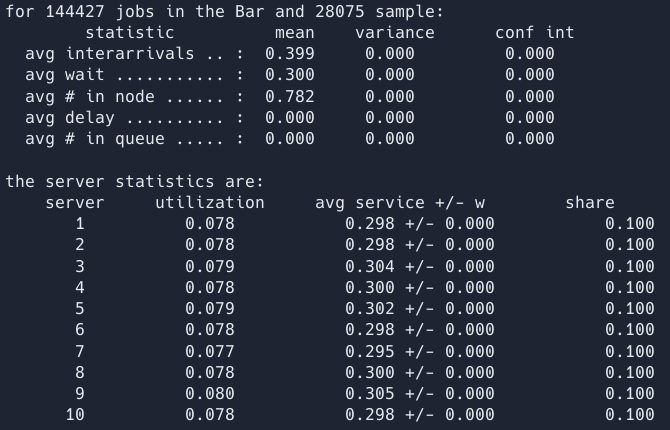
\includegraphics[width=\textwidth]{rho_services_b}
\end{minipage}
\hfill
\begin{minipage}{0.4\textwidth}
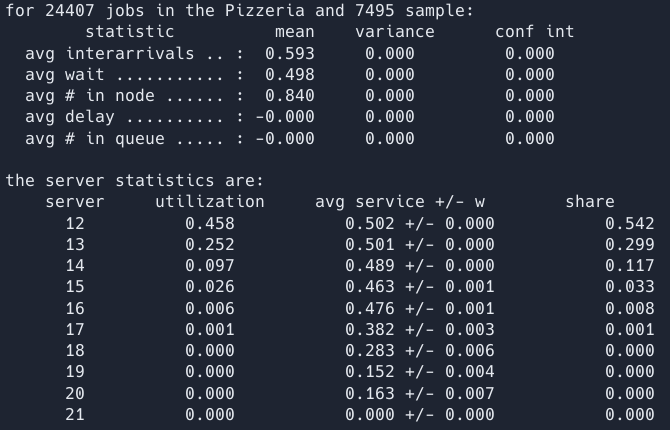
\includegraphics[width=\textwidth]{rho_services_p}
\end{minipage}
\hspace*{\fill}
\bigskip

Dai risultati relativi all'utilizzazione, al tempo medio di servizio e allo \textit{share}, emerge chiaramente il rispetto delle specifiche prestabilite: infatti tutti i server di tipo "B" presentano valori simili per tutte le grandezze in esame mentre per i server di tipo "P" si osserva una tendenza al decremento dei valori all'aumentare dell'indice del server.

\subsection{Conclusione}

Sulla base dei risultati ottenuti dagli esperimenti condotti, è possibile trarre la conclusione che il simulatore dimostra una buona capacità di adattamento ai cambiamenti di configurazione. Inoltre, utilizzando un numero sufficiente di job nella simulazione, si osserva che il simulatore è in grado di produrre risultati coerenti con le previsioni teoriche. Ciò suggerisce che il simulatore è fedele al modello del sistema in esame e offre una rappresentazione affidabile del comportamento del sistema stesso


\section{Validazione}
Durante il processo di validazione si sono riscontrate delle sfide significative nell'utilizzo dell'analisi a orizzonte finito, principalmente dovute al numero limitato di job processati. Questa limitazione ha comportato un campione statistico ridotto e, di conseguenza, una maggiore variabilità nei risultati osservati. In altre parole, la variabilità è emersa come una problematica a causa della limitata quantità di dati disponibili. È importante notare che, in un contesto in cui avessimo processato un numero significativamente maggiore di job in ogni run, la variabilità non avrebbe avuto un impatto significativo. \\

Per validare il modello, quindi, si è deciso di adottare un'analisi a orizzonte infinito in modo da ottenere risultati più stabili. In questa fase verifichiamo se, per ciascuna fascia oraria, le statistiche generate dal nostro simulatore convergono ai valori reali. 

\subsection{Analisi a orizzonte infinito}
Per condurre un'analisi a orizzonte infinito, è necessario utilizzare i seguenti comandi:

\begin{itemize}
  \item \key{make infinite-week}: esegue \key{python3 simulation.py -ih -s 123 -of week}. Effettua l'analisi per il giorno lavorativo della settimana.
  \item \key{make infinite-weekend}: esegue \texttt{python3 simulation.py -ih -s 123 -wed -of weekend}. Effettua l'analisi per il fine settimana.
\end{itemize}

È fondamentale notare che, prima di eseguire questi comandi, è consigliabile eliminare eventuali file di output CSV già presenti al fine di evitare confusione nei risultati.\\

Per determinare i parametri dell'analisi, è possibile specificare il flag \key{-fb THRESHOLD}, il quale consente di determinare dinamicamente il numero di campioni da raccogliere per ogni batch. Il parametro \key{THRESHOLD} specifica che il valore di autocorrelazione per lag \key{j = 1} di ogni statistica non deve superare quel valore. Utilizzando \key{k = 128} batches, ciascuno con \key{b = 1024} campioni, l'autocorrelazione per lag \texttt{j = 1} è inferiore a \key{0.2}, contribuendo così alla stabilità e all'affidabilità dei risultati.\\

L'analisi viene condotta per ciascun tipo di richiesta e per ciascuna statistica di interesse, coprendo tutte le fasce orarie sia nei giorni lavorativi che nei giorni del fine settimana. I risultati vengono presentati in forma tabellare e grafica; in particolare, nelle tabelle si riportano i risultati sperimentali ottenuti mediando su tutti i batch con un intervallo di confidenza al 95\%.\\


\begin{adjustbox}{width=\textwidth}
\centering
\begin{tabular}{ |c|c|c|c|c|c|c|c| }
\cline{2-7}
\multicolumn{1}{c}{} & \multicolumn{6}{|c|}{\cellcolor{cellcolor}\textit{B type - Interarrivals}}\\
\cline{2-7}
\multicolumn{1}{c|}{} & \cellcolor{cellcolor}Slot & \cellcolor{cellcolor}Risultato teorico & \cellcolor{cellcolor}Risultato sperimentale &  \cellcolor{cellcolor}Media nell'intervallo &
\cellcolor{cellcolor}Errore & \cellcolor{cellcolor}Link all'immagine\\
\cline{2-7}
\noalign{\vspace{0.5ex}}
\hline
\cellcolor{cellcolor}& 0 & 2.000 min & 2.000 $\pm$ 0.014 min & \checkmark & & \hyperlink{interarrivo infinito week slot 0}{link}  \\ 
\cline{2-7}
\cellcolor{cellcolor}& 1 & 4.762 min & 4.950 $\pm$ 0.389 min & \checkmark & & \hyperlink{interarrivo infinito week slot 1}{link}\\
\cline{2-7}
\cellcolor{cellcolor}& 3 & 2.381 min & 2.614 $\pm$ 0.477 min & \checkmark & & \hyperlink{interarrivo infinito week slot 3}{link}\\
\cline{2-7}
\cellcolor{cellcolor}& 4 & 4.762 min & 5.154 $\pm$ 0.811 min & \checkmark & & \hyperlink{interarrivo infinito week slot 4}{link}\\
\cline{2-7}
\multirow{-6}{*}{\rotatebox[origin=c]{90}{\cellcolor{cellcolor}Week}} & 5 & 5.882 min & 6.217 $\pm$ 0.074 min & \checkmark & & \hyperlink{interarrivo infinito week slot 5}{link}\\
\hline
\hline
\cellcolor{cellcolor}& 0 & 2.000 min & 2.000 $\pm$ 0.014 min & \checkmark & & \hyperlink{interarrivo infinito weekend slot 0}{link}\\ 
\cline{2-7}
\cellcolor{cellcolor}& 1 & 2.941 min & 3.091 $\pm$ 0.322 min & \checkmark & &\hyperlink{interarrivo infinito weekend slot 1}{link}\\
\cline{2-7}
\cellcolor{cellcolor}& 3 & 1.333 min & 1.460 $\pm$ 0.259 min & \checkmark & & \hyperlink{interarrivo infinito weekend slot 3}{link}\\
\cline{2-7}
\cellcolor{cellcolor}& 4 & 2.667 min & 2.794 $\pm$ 0.268 min & \checkmark & & \hyperlink{interarrivo infinito weekend slot 4}{link}\\
\cline{2-7}
\multirow{-6}{*}{\rotatebox[origin=c]{90}{\cellcolor{cellcolor}Weekend}} & 5 & 2.941 min & 3.065 $\pm$ 0.285 min & \checkmark & & \hyperlink{interarrivo infinito weekend slot 5}{link}\\
\hline
\end{tabular}
\end{adjustbox}
\bigskip

\begin{adjustbox}{width=\textwidth}
\centering
\begin{tabular}{ |c|c|c|c|c|c|c|c| }
\cline{2-7}
\multicolumn{1}{c}{} & \multicolumn{6}{|c|}{\cellcolor{cellcolor}\textit{B type - Waits}}\\
\cline{2-7}
\multicolumn{1}{c|}{} & \cellcolor{cellcolor}Slot & \cellcolor{cellcolor}Risultato teorico & \cellcolor{cellcolor}Risultato sperimentale &  \cellcolor{cellcolor}Media nell'intervallo &
\cellcolor{cellcolor}Errore & \cellcolor{cellcolor}Link all'immagine \\
\cline{2-7}
\noalign{\vspace{0.5ex}}
\hline
\cellcolor{cellcolor}& 0 & 2.667 min & 2.665 $\pm$ 0.035 min & \checkmark & & \hyperlink{attesa infinita week slot 0}{link} \\ 
\cline{2-7}
\cellcolor{cellcolor}& 1 & 2.092 min & 2.083 $\pm$ 0.018 min & \checkmark & & \hyperlink{attesa infinita week slot 1}{link}\\ 
\cline{2-7}
\cellcolor{cellcolor}& 3 & 2.428 min & 2.440 $\pm$ 0.027 min & \checkmark & & \hyperlink{attesa infinita week slot 3}{link}\\ 
\cline{2-7}
\cellcolor{cellcolor}& 4 & 2.092 min & 2.086 $\pm$ 0.021 min & \checkmark & & \hyperlink{attesa infinita week slot 4}{link} \\ 
\cline{2-7}
\multirow{-6}{*}{\rotatebox[origin=c]{90}{\cellcolor{cellcolor}Week}} & 5 & 2.060 min & 2.067 $\pm$ 0.023 min & \checkmark & & \hyperlink{attesa infinita week slot 5}{link}\\ 
\hline
\hline
\cellcolor{cellcolor}& 0 & 2.667 min & 2.665 $\pm$ 0.035 min & \checkmark & & \hyperlink{attesa infinita weekend slot 0}{link}\\ 
\cline{2-7}
\cellcolor{cellcolor}& 1 & 2.261 min & 2.257 $\pm$ 0.024 min & \checkmark & &\hyperlink{attesa infinita weekend slot 1}{link}\\ 
\cline{2-7}
\cellcolor{cellcolor}& 3 & 4.571 min & 4.499 $\pm$ 0.115 min & \checkmark & & \hyperlink{attesa infinita weekend slot 3}{link}\\ 
\cline{2-7}
\cellcolor{cellcolor}& 4 & 2.327 min & 2.339 $\pm$ 0.031 min & \checkmark & & \hyperlink{attesa infinita weekend slot 4}{link}\\ 
\cline{2-7}
\multirow{-6}{*}{\rotatebox[origin=c]{90}{\cellcolor{cellcolor}Weekend}} & 5 & 2.261 min & 2.246 $\pm$ 0.025 min & \checkmark & & \hyperlink{attesa infinita weekend slot 5}{link}\\ 
\hline
\end{tabular}
\end{adjustbox}
\bigskip

\begin{adjustbox}{width=\textwidth}
\centering
\begin{tabular}{ |c|c|c|c|c|c|c|c| }
\cline{2-7}
\multicolumn{1}{c}{} & \multicolumn{6}{|c|}{\cellcolor{cellcolor}\textit{B type - Num. in the nodes}}\\
\cline{2-7}
\multicolumn{1}{c|}{} & \cellcolor{cellcolor}Slot & \cellcolor{cellcolor}Risultato teorico & \cellcolor{cellcolor}Risultato sperimentale &  \cellcolor{cellcolor}Media nell'intervallo &
\cellcolor{cellcolor}Errore & \cellcolor{cellcolor}Link all'immagine\\
\cline{2-7}
\noalign{\vspace{0.5ex}}
\hline
\cellcolor{cellcolor}& 0 & 1.333 min & 1.336 $\pm$ 0.021 min & \checkmark & & \hyperlink{centro infinito week slot 0}{link}  \\ 
\cline{2-7}
\cellcolor{cellcolor}& 1 & 0.439 min & 0.440 $\pm$ 0.006 min & \checkmark & & \hyperlink{centro infinito week slot 1}{link}\\
\cline{2-7}
\cellcolor{cellcolor}& 3 & 1.020 min & 1.031 $\pm$ 0.016 min & \checkmark & & \hyperlink{centro infinito week slot 3}{link}\\
\cline{2-7}
\cellcolor{cellcolor}& 4 & 0.439 min & 0.440 $\pm$ 0.007 min & \checkmark & & \hyperlink{centro infinito week slot 4}{link}\\
\cline{2-7}
\multirow{-6}{*}{\rotatebox[origin=c]{90}{\cellcolor{cellcolor}Week}} & 5 & 0.350 min & 0.355 $\pm$ 0.005 min & \checkmark & & \hyperlink{centro infinito week slot 5}{link}\\
\hline
\hline
\cellcolor{cellcolor}& 0 & 1.333 min & 1.336 $\pm$ 0.021 min & \checkmark & & \hyperlink{centro infinito weekend slot 0}{link}\\ 
\cline{2-7}
\cellcolor{cellcolor}& 1 & 0.769 min & 0.773 $\pm$ 0.011 min & \checkmark & &\hyperlink{centro infinito weekend slot 1}{link}\\
\cline{2-7}
\cellcolor{cellcolor}& 3 & 3.429 min & 3.399 $\pm$ 0.095 min & \checkmark & & \hyperlink{centro infinito weekend slot 3}{link}\\
\cline{2-7}
\cellcolor{cellcolor}& 4 & 0.873 min & 0.881 $\pm$ 0.014 min & \checkmark & & \hyperlink{centro infinito weekend slot 4}{link}\\
\cline{2-7}
\multirow{-6}{*}{\rotatebox[origin=c]{90}{\cellcolor{cellcolor}Weekend}} & 5 & 0.769 min & 0.769 $\pm$ 0.011 min & \checkmark & & \hyperlink{centro infinito weekend slot 5}{link}\\
\hline
\end{tabular}
\end{adjustbox}
\bigskip

\begin{adjustbox}{width=\textwidth}
\centering
\begin{tabular}{ |c|c|c|c|c|c|c|c| }
\cline{2-7}
\multicolumn{1}{c}{} & \multicolumn{6}{|c|}{\cellcolor{cellcolor}\textit{B type - Delays}}\\
\cline{2-7}
\multicolumn{1}{c|}{} & \cellcolor{cellcolor}Slot & \cellcolor{cellcolor}Risultato teorico & \cellcolor{cellcolor}Risultato sperimentale &  \cellcolor{cellcolor}Media nell'intervallo &
\cellcolor{cellcolor}Errore & \cellcolor{cellcolor}Link all'immagine\\
\cline{2-7}
\noalign{\vspace{0.5ex}}
\hline
\cellcolor{cellcolor}& 0 & 0.667 min & 0.671 $\pm$ 0.027 min & \checkmark & & \hyperlink{ritardo infinito week slot 0}{link}  \\ 
\cline{2-7}
\cellcolor{cellcolor}& 1 & 0.092 min & 0.100 $\pm$ 0.006 min & \xmark & 0.002 & \hyperlink{ritardo infinito week slot 1}{link}\\
\cline{2-7}
\cellcolor{cellcolor}& 3 & 0.428 min & 0.455 $\pm$ 0.019 min & \xmark & 0.008 & \hyperlink{ritardo infinito week slot 3}{link}\\
\cline{2-7}
\cellcolor{cellcolor}& 4 & 0.092 min & 0.098 $\pm$ 0.007 min & \checkmark & & \hyperlink{ritardo infinito week slot 4}{link}\\
\cline{2-7}
\multirow{-6}{*}{\rotatebox[origin=c]{90}{\cellcolor{cellcolor}Week}} & 5 & 0.060 min & 0.072 $\pm$ 0.007 min & \xmark & 0.005 & \hyperlink{ritardo infinito week slot 5}{link}\\
\hline
\hline
\cellcolor{cellcolor}& 0 & 0.667 min & 0.671 $\pm$ 0.027 min & \checkmark & & \hyperlink{ritardo infinito weekend slot 0}{link}\\ 
\cline{2-7}
\cellcolor{cellcolor}& 1 & 0.261 min & 0.268 $\pm$ 0.014 min & \checkmark & &\hyperlink{ritardo infinito weekend slot 1}{link}\\
\cline{2-7}
\cellcolor{cellcolor}& 3 & 2.571 min & 2.519 $\pm$ 0.108 min & \checkmark & & \hyperlink{ritardo infinito weekend slot 3}{link}\\
\cline{2-7}
\cellcolor{cellcolor}& 4 & 0.327 min & 0.342 $\pm$ 0.020 min & \checkmark &  & \hyperlink{ritardo infinito weekend slot 4}{link}\\
\cline{2-7}
\multirow{-6}{*}{\rotatebox[origin=c]{90}{\cellcolor{cellcolor}Weekend}} & 5 & 0.261 min & 0.265 $\pm$ 0.014 min & \checkmark & & \hyperlink{ritardo infinito weekend slot 5}{link}\\
\hline
\end{tabular}
\end{adjustbox}
\bigskip

\begin{adjustbox}{width=\textwidth}
\centering
\begin{tabular}{ |c|c|c|c|c|c|c|c| }
\cline{2-7}
\multicolumn{1}{c}{} & \multicolumn{6}{|c|}{\cellcolor{cellcolor}\textit{B type - Num. in the queue}}\\
\cline{2-7}
\multicolumn{1}{c|}{} & \cellcolor{cellcolor}Slot & \cellcolor{cellcolor}Risultato teorico & \cellcolor{cellcolor}Risultato sperimentale &  \cellcolor{cellcolor}Media nell'intervallo &
\cellcolor{cellcolor}Errore & \cellcolor{cellcolor}Link all'immagine\\
\cline{2-7}
\noalign{\vspace{0.5ex}}
\hline
\cellcolor{cellcolor}& 0 & 0.333 min & 0.339 $\pm$ 0.015 min & \checkmark & & \hyperlink{coda infinita week slot 0}{link}  \\ 
\cline{2-7}
\cellcolor{cellcolor}& 1 & 0.019 min & 0.021 $\pm$ 0.001 min & \xmark & 0.001 & \hyperlink{coda infinita week slot 1}{link}\\
\cline{2-7}
\cellcolor{cellcolor}& 3 & 0.180 min & 0.194 $\pm$ 0.005 min & \xmark &0.009  & \hyperlink{coda infinita week slot 3}{link}\\
\cline{2-7}
\cellcolor{cellcolor}& 4 & 0.019 min & 0.021 $\pm$ 0.001 min & \xmark & 0.001 & \hyperlink{coda infinita week slot 4}{link}\\
\cline{2-7}
\multirow{-6}{*}{\rotatebox[origin=c]{90}{\cellcolor{cellcolor}Week}} & 5 & 0.010 min & 0.013 $\pm$ 0.001 min & \xmark & 0.002 & \hyperlink{coda infinita week slot 5}{link}\\
\hline
\hline
\cellcolor{cellcolor}& 0 & 0.333 min & 0.339 $\pm$ 0.015 min & \checkmark & & \hyperlink{coda infinita weekend slot 0}{link}\\ 
\cline{2-7}
\cellcolor{cellcolor}& 1 & 0.089 min & 0.093 $\pm$ 0.005 min & \checkmark & &\hyperlink{coda infinita weekend slot 1}{link}\\
\cline{2-7}
\cellcolor{cellcolor}& 3 & 1.929 min & 1.910 $\pm$ 0.087 min & \checkmark & & \hyperlink{coda infinita weekend slot 3}{link}\\
\cline{2-7}
\cellcolor{cellcolor}& 4 & 0.123 min & 0.130 $\pm$ 0.008 min & \checkmark &  & \hyperlink{coda infinita weekend slot 4}{link}\\
\cline{2-7}
\multirow{-6}{*}{\rotatebox[origin=c]{90}{\cellcolor{cellcolor}Weekend}} & 5 & 0.089 min & 0.092 $\pm$ 0.005 min & \checkmark & & \hyperlink{coda infinita weekend slot 5}{link}\\
\hline
\end{tabular}
\end{adjustbox}
\bigskip

\begin{adjustbox}{width=\textwidth}
\centering
\begin{tabular}{ |c|c|c|c|c|c|c| }
\cline{2-7}
\multicolumn{1}{c}{} & \multicolumn{6}{|c|}{\cellcolor{cellcolor}\textit{P type - all statistics in the slot}}\\
\cline{2-7}
\multicolumn{1}{c|}{} & \cellcolor{cellcolor}Statistica & \cellcolor{cellcolor}Risultato teorico & \cellcolor{cellcolor}Risultato sperimentale &  \cellcolor{cellcolor}Media nell'intervallo &
\cellcolor{cellcolor}Errore & \cellcolor{cellcolor}Link all'immagine \\
\cline{2-7}
\noalign{\vspace{0.5ex}}
\hline
\cellcolor{cellcolor}& Interarrivo & 5.882 min & 6.145 $\pm$ 0.499 min & \checkmark & & \hyperlink{interarrivo infinito week P}{link} \\ 
\cline{2-7}
\cellcolor{cellcolor}& Attesa & 3.209 min & 3.223 $\pm$ 0.038 min & \checkmark & & \hyperlink{attesa infinita week P}{link} \\
\cline{2-7}
\cellcolor{cellcolor}& Num. nel nodo & 0.545 min & 0.548 $\pm$ 0.009 min & \checkmark & & \hyperlink{centro infinito week P}{link} \\
\cline{2-7}
\cellcolor{cellcolor}& Ritardo & 0.209 min & 0.229 $\pm$ 0.017 min & \xmark & 0.003 & \hyperlink{ritardo infinito week P}{link} \\
\cline{2-7}
\multirow{-6}{*}{\rotatebox[origin=c]{90}{\cellcolor{cellcolor}Week}} & Num. in coda & 0.035 min & 0.040 $\pm$ 0.003 min & \xmark & 0.002	 & \hyperlink{coda infinita week P}{link}\\
\hline
\hline
\cellcolor{cellcolor}& Interarrivo & 2.000 min & 2.114 $\pm$ 0.228 min & \checkmark & & \hyperlink{interarrivo infinito weekend P}{link} \\ 
\cline{2-7}
\cellcolor{cellcolor}& Attesa & 6.867 min & 6.979 $\pm$ 0.281 min & \checkmark & & \hyperlink{attesa infinita weekend P}{link}\\
\cline{2-7}
\cellcolor{cellcolor}& Num. nel nodo & 3.429 min & 3.505 $\pm$ 0.150 min & \checkmark & & \hyperlink{centro infinito weekend P}{link} \\
\cline{2-7}
\cellcolor{cellcolor}& Ritardo & 3.857 min & 3.985 $\pm$ 0.267 min & \checkmark & & \hyperlink{ritardo infinito weekend P}{link} \\
\cline{2-7}
\multirow{-6}{*}{\rotatebox[origin=c]{90}{\cellcolor{cellcolor}Weekend}} & Num. in coda & 1.929 min & 2.010 $\pm$ 0.139 min & \checkmark & & \hyperlink{coda infinita weekend P}{link} \\
\hline
\end{tabular}
\end{adjustbox}
\bigskip

L'analisi a orizzonte infinito ha dimostrato che la maggior parte dei risultati converge in modo affidabile ai valori teorici previsti per il caso di studio in esame, confermando così l'accuratezza del nostro simulatore nel rappresentare il comportamento del sistema in uno stato stazionario. Tuttavia, un aspetto interessante emerge quando ripetiamo l'analisi utilizzando un seme iniziale diverso, specificamente il seme \key{12345}, con il comando \key{make clean infinite-weekend SEED=12345}. In questo caso, notiamo che la maggior parte degli errori viene azzerata, e gli altri risultano notevolmente ridotti. Questo suggerisce che il caso con il seme iniziale pari a \key{123} potrebbe essere considerato come un caso particolarmente sfortunato per l'analisi delle statistiche.\\

È interessante notare anche che nei casi in cui la frequenza di arrivo è leggermente più alta, come nel fine settimana, questi errori risultano azzerati anche con lo stesso seme \key{123}. Ciò evidenzia come la bassa frequenza di arrivo possa influenzare la precisione delle stime di queste grandezze, persino nell'analisi a orizzonte infinito. 

\section{Analisi dei costi e dei guadagni}
Per effettuare l'analisi dei costi e dei guadagni sul caso di studio in esame è stata eseguita un'analisi a orizzonte finito che, seppur poco rappresentativa in ambito di validazione, è quella che permette effettivamente di valutare le entrate e le uscite per un sistema con queste specifiche. 

\subsection{Analisi a orizzonte finito}
Utilizzando questo approccio, il sistema è stato simulato per un periodo di 16 ore lavorative effettive, tenendo conto delle variazioni nei tassi di arrivo durante le diverse fasce orarie. Affinché l'analisi a orizzonte infinito sia affidabile, è fondamentale che lo stato iniziale e quello finale del sistema siano identici. Nel contesto specifico, la simulazione inizia e termina senza che ci siano richieste nel sistema.\\

Per ottenere risultati robusti per l'analisi a orizzonte infinito, la simulazione di una giornata lavorativa è stata eseguita per 1024 iterazioni. In ciascuna di esse sono state ripristinate tutte le statistiche mentre lo stato del generatore di numeri casuali è stato mantenuto inalterato. Questo approccio assicura l'indipendenza tra le diverse esecuzioni.\\

Anche in questo caso, è stata condotta un'analisi separata per ciascun tipo di richiesta, considerando i tempi di risposta con e senza l'introduzione del fattore gaussiano. I risultati sono stati presentati in forma tabellare e grafica, con le tabelle che riportano i risultati sperimentali ottenuti mediante la media di tutti i \textit{run}, con un intervallo di confidenza del 95\%.
\bigskip

\begin{adjustbox}{width=\textwidth}
\centering
\begin{tabular}{ |c|c|c|c|c|c|c|c|c| }
\cline{2-8}
\multicolumn{1}{c}{} & \multicolumn{7}{|c|}{\cellcolor{cellcolor}\textit{Analisi senza fattore gaussiano}}\\
\cline{2-8}
\multicolumn{1}{c|}{} & \cellcolor{cellcolor}Statistica & \cellcolor{cellcolor}Risultato teorico & \cellcolor{cellcolor}Risultato sperimentale &  \cellcolor{cellcolor}Media nell'intervallo &
\cellcolor{cellcolor}Errore & \cellcolor{cellcolor}Link all'immagine & \cellcolor{cellcolor} Rispetta QoS\\
\cline{2-8}
\noalign{\vspace{0.5ex}}
\cline{1-8}
\cellcolor{cellcolor}& \makecell{Attesa di\\ tipo B} & 2.251 min & 2.455 $\pm$ 0.023 min & \xmark & 0.181 & \hyperlink{attesa finita week B no gau}{link} & \checkmark \\ 
\cline{2-8}
\multirow{-3}{*}{\rotatebox[origin=c]{90}{\cellcolor{cellcolor}Week}} & \makecell{Attesa di\\ tipo P} & 3.209 min & 3.212 $\pm$ 0.049 min & \checkmark & & \hyperlink{attesa finita week P no gau}{link} & \checkmark \\

\cline{1-8}
\noalign{\vspace{0.5ex}}
\cline{1-8}

\cellcolor{cellcolor}&\makecell{Attesa di\\ tipo B} & 2.524 min & 2.761 $\pm$ 0.032 min & \xmark & 0.205	 & \hyperlink{attesa finita weekend B no gau}{link} & \checkmark \\
\cline{2-8}
\multirow{-3}{*}{\rotatebox[origin=c]{90}{\cellcolor{cellcolor}Weekend}} & \makecell{Attesa di\\ tipo P} & 6.857 min & 5.813 $\pm$ 0.150 min & \xmark & 0.894 & \hyperlink{attesa finita weekend P no gau}{link} & \checkmark\\
\cline{1-8}

\end{tabular}
\end{adjustbox}
\bigskip

\begin{adjustbox}{width=\textwidth}
\centering
\begin{tabular}{ |c|c|c|c|c|c|c|c|c| }
\cline{2-8}
\multicolumn{1}{c}{} & \multicolumn{7}{|c|}{\cellcolor{cellcolor}\textit{Analisi con fattore gaussiano}}\\
\cline{2-8}
\multicolumn{1}{c|}{} & \cellcolor{cellcolor}Statistica & \cellcolor{cellcolor}Risultato teorico & \cellcolor{cellcolor}Risultato sperimentale &  \cellcolor{cellcolor}Media nell'intervallo &
\cellcolor{cellcolor}Errore & \cellcolor{cellcolor}Link all'immagine & \cellcolor{cellcolor} Rispetta QoS\\
\cline{2-8}
\noalign{\vspace{0.5ex}}
\cline{1-8}
\cellcolor{cellcolor}& \makecell{Attesa di\\ tipo B} & 2.251 min & 2.184 $\pm$ 0.027 min & \xmark & 0.040 & \hyperlink{attesa finita week B gau}{link} & \checkmark \\ 
\cline{2-8}
\multirow{-3}{*}{\rotatebox[origin=c]{90}{\cellcolor{cellcolor}Week}} & \makecell{Attesa di\\ tipo P} & 3.209 min & 3.082 $\pm$ 0.078 min & \xmark & 0.049 & \hyperlink{attesa finita week P gau}{link} & \checkmark \\

\cline{1-8}
\noalign{\vspace{0.5ex}}
\cline{1-8}

\cellcolor{cellcolor}&\makecell{Attesa di\\ tipo B} & 2.524 min & 2.987 $\pm$ 0.075 min & \xmark & 0.388	 & \hyperlink{attesa finita weekend B gau}{link} & \checkmark \\
\cline{2-8}
\multirow{-3}{*}{\rotatebox[origin=c]{90}{\cellcolor{cellcolor}Weekend}} & \makecell{Attesa di\\ tipo P} & 6.857 min & 3.209 $\pm$ 0.056 min & \xmark & 3.592 & \hyperlink{attesa finita weekend P gau}{link} & \checkmark\\
\cline{1-8}

\end{tabular}
\end{adjustbox}
\bigskip

Come previsto dalle osservazioni precedenti, il valore teorico raramente rientra nell'intervallo di confidenza della statistica sperimentale. Tuttavia, con la configurazione che prevede $m_B = 2$, tutti i requisiti di Qualità del Servizio (QoS) sono costantemente rispettati. È importante notare che la scelta di $m_B = 1$ non rende il sistema stabile nella prima fascia oraria, in cui $\lambda_B = 0.5 j/min$. Per un unico server, infatti:
\[
	\rho = \lambda E(S) = 0.5\ j/min \cdot 2\ min = 1
\]

Quindi, la scelta di $m_B = 2$ appare come la più logica, in quanto rappresenta il valore minimo di $m$ che garantisce il rispetto dei QoS.\\

Inoltre, anche le utilizzazioni dei server sono accettabili e vengono riportate insieme ai valori delle altre grandezze nelle seguenti immagini:

\begin{minipage}{0.5\textwidth}
\begin{figure}[H]
\centering
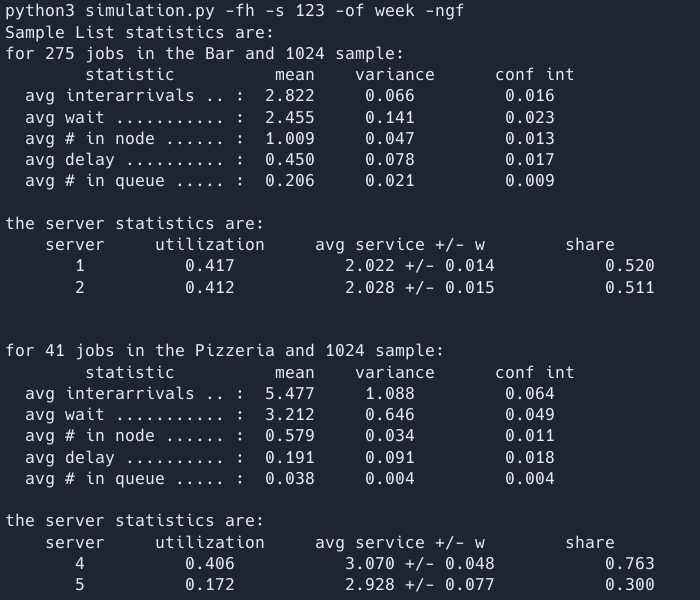
\includegraphics[width=0.8\textwidth]{finite_horizont_output_week_ngf}

\textit{Week day - senza fattore gaussiano}
\end{figure}
\end{minipage}
\begin{minipage}{0.5\textwidth}
\begin{figure}[H]
\centering
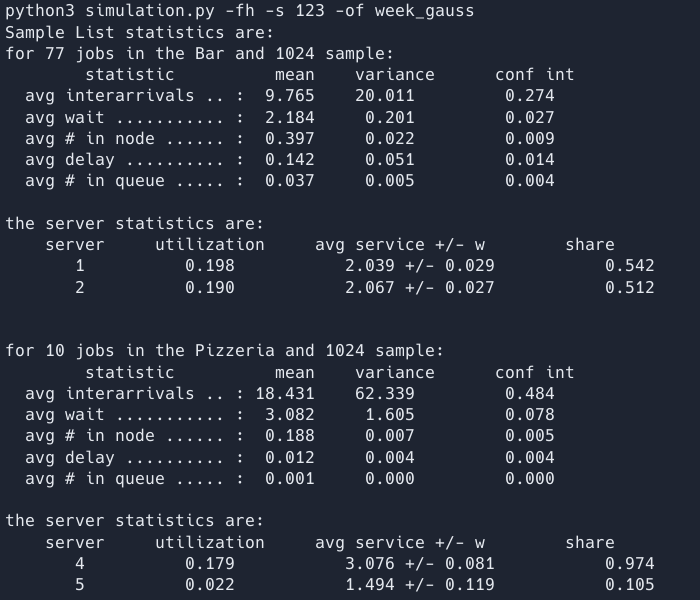
\includegraphics[width=0.8\textwidth]{finite_horizont_output_week_g}

\textit{Week day - con fattore gaussiano}
\end{figure}
\end{minipage}

\begin{minipage}{0.5\textwidth}
\begin{figure}[H]
\centering
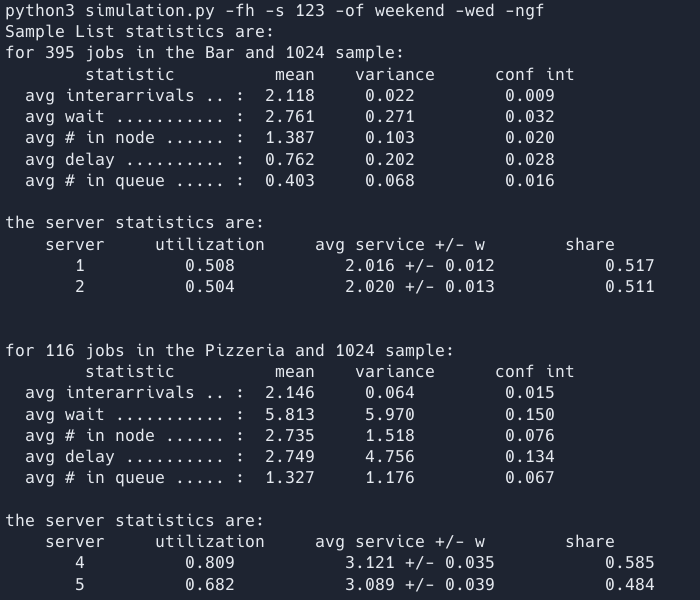
\includegraphics[width=0.8\textwidth]{finite_horizont_output_weekend_ngf}

\textit{Weekend day - senza fattore gaussiano}
\end{figure}
\end{minipage}
\begin{minipage}{0.5\textwidth}
\begin{figure}[H]
\centering
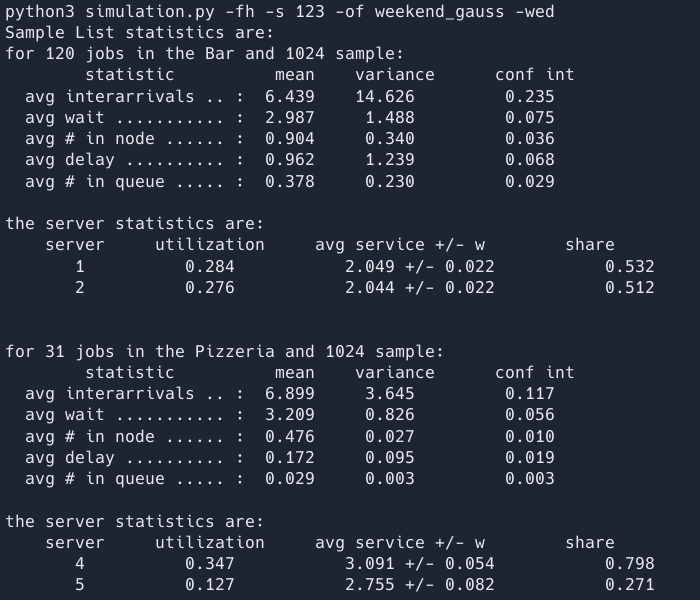
\includegraphics[width=0.8\textwidth]{finite_horizont_output_weekend_g}

\textit{Weekend day - con fattore gaussiano}
\end{figure}
\end{minipage}
\bigskip


Il numero di job presente nelle immagini precedenti rappresenta la media dei job processati in diverse esecuzioni e verrà utilizzato successivamente come numero di richieste giornaliere nell'analisi dei costi. I calcoli sono stati effettuati su base mensile (4 settimane), e quindi le grandezze giornaliere sono state convertite di conseguenza. Le configurazioni utilizzate sono quelle di default presenti nel file \key{configurations/Config.py}.


\subsection{Analisi delle spese}
\begin{table}[H]
\centering
\begin{tabular}{|c|c|c|}
\hline
\cellcolor{cellcolor}Spesa & \cellcolor{cellcolor}Valore & \cellcolor{cellcolor}Contributo mensile \\
\hline
\hline
Baristi & $40,00 \mbox{\euro}$ al giorno per barista & $40,00 \cdot 28 \cdot 2 = 2.240,00\ \mbox{\euro}$ al mese \\
\hline
Pizzaiolo & $40,00 \mbox{\euro}$ al giorno & $50,00 \cdot 28 = 1400\ \mbox{\euro}$  al mese\\
\hline
Bollette & $2.750,00 \mbox{\euro}$ al mese & $2.750,00 \mbox{\euro}$ al mese \\
\hline
Affitto & $1.500,00 \mbox{\euro}$ al mese & $1.500,00 \mbox{\euro}$ al mese\\
\hline
Fornitori & $2.000,00 \mbox{\euro}$ al mese & $2.000,00 \mbox{\euro}$ al mese\\
\hline
\hline
\multicolumn{2}{|c|}{Totale} & \cellcolor{red!40} $12.970,00 \mbox{\euro}$\\
\hline

\end{tabular}
\end{table}

\subsection{Analisi dei guadagni}

\subsubsection{Senza fattore gaussiano}
\begin{adjustbox}{width=\textwidth}
\begin{tabular}{|c|c|c|c|c|c|}
\hline
\cellcolor{cellcolor}Tipo richiesta & \cellcolor{cellcolor}Richieste \textit{week} & \cellcolor{cellcolor}Richieste \textit{weekend} & \cellcolor{cellcolor}Guadagno & \cellcolor{cellcolor}Contributo mensile &
\cellcolor{cellcolor} Con IVA al 10\% \\
\hline
\hline
Tipo B & 275 & 395 & $5,00\ \mbox{\euro}$ a richiesta & \makecell{$ (275 \cdot 5 + 395 \cdot 2 )\cdot 5,00 \cdot 4 =$ \\ $43.300,00 \mbox{\euro}$ al mese } & $ 43.300,00 \cdot 0.9 = 38.970,00 \mbox{\euro}$ \\
\hline
Tipo P & 41 & 116 & $10\ \mbox{\euro}$ a richiesta & \makecell{$ (41 \cdot 5 + 116 \cdot 2 )\cdot 10,00 \cdot 4 =$ \\ $17.480,00\ \mbox{\euro}$ al mese } & $ 17480 \cdot 0.9 = 15.732,00 \mbox{\euro}$ \\

\hline
\hline

%\multicolumn{2}{|c|}{Totale} & \cellcolor{red!40} \textcolor[RGB]{230,10,10}{12970 $\mbox{\euro}$}\\
\multicolumn{5}{|c|}{Totale} & \cellcolor{green!40} $54.702,00 \mbox{\euro}$\\
\hline

\end{tabular}
\end{adjustbox}
\bigskip


Il guadagno netto mensile risulta essere:
\[
	54.702,00 - 12.970,00 = 41.732,00 \mbox{\euro}
\]

\subsubsection{Con fattore gaussiano}
\begin{adjustbox}{width=\textwidth}
\begin{tabular}{|c|c|c|c|c|c|}
\hline
\cellcolor{cellcolor}Tipo richiesta & \cellcolor{cellcolor}Richieste \textit{week} & \cellcolor{cellcolor}Richieste \textit{weekend} & \cellcolor{cellcolor}Guadagno & \cellcolor{cellcolor}Contributo mensile &
\cellcolor{cellcolor} Con IVA al 10\% \\
\hline
\hline
Tipo B & 77 & 120 & $5,00\ \mbox{\euro}$ a richiesta & \makecell{$ (77 \cdot 5 + 120 \cdot 2 )\cdot 5,00 \cdot 4 =$ \\ $12.500,00 \mbox{\euro}$ al mese } & $ 12.500,00 \cdot 0.9 = 11.250,00 \mbox{\euro}$ \\
\hline
Tipo P & 10 & 31 & $10,00\ \mbox{\euro}$ a richiesta & \makecell{$ (10 \cdot 5 + 31 \cdot 2 )\cdot 10,00 \cdot 4 =$ \\ $4.480,00 \mbox{\euro}$ al mese } & $ 4.480,00 \cdot 0.9 = 4.032,00 \mbox{\euro}$ \\

\hline
\hline

\multicolumn{5}{|c|}{Totale} & \cellcolor{green!40} $15.282,00 \mbox{\euro}$\\
\hline

\end{tabular}
\end{adjustbox}
\bigskip

Il guadagno netto mensile risulta essere:
\[
	15.282,00 - 12.970,00 = 2.312,00 \mbox{\euro}
\]



\subsection{Conclusioni}
Nel caso in cui non si utilizzi la normalizzazione gaussiana, si osserva un guadagno netto mensile di 41.732 euro. Tuttavia, questo valore sembra essere ottimistico poiché non tiene conto di alcuna concentrazione delle richieste nelle diverse fasce orarie. Dall'altro lato, nel caso in cui si utilizzi la normalizzazione gaussiana, il guadagno mensile si riduce a 2.312 euro.

I risultati suggeriscono che la seconda cifra sia più realistica e rappresenti meglio la situazione effettiva, dato che l'arrivo delle richieste tende a concentrarsi maggiormente nelle diverse fasce orarie.

In conclusione, la scelta di utilizzare la normalizzazione gaussiana sembra più aderente alla realtà operativa e produce una stima più conservativa dei guadagni mensili, che si attesta a 2.312 euro. Questo valore riflette meglio le condizioni operative del sistema in cui le richieste sono distribuite in modo più realistico nel corso della giornata.



\section{Immagini}

\target{rappresentazione grafica gaussiane}
\subsection{Distribuzioni gaussiane per gli arrivi}
\[
y=\frac{1}{\sqrt{2\pi}\sigma}e^\frac{-(x-\mu)^2}{2\sigma^2}
\]

\target{distribuzione gaussiana 7-11}
\begin{figure}[H]
\centering 
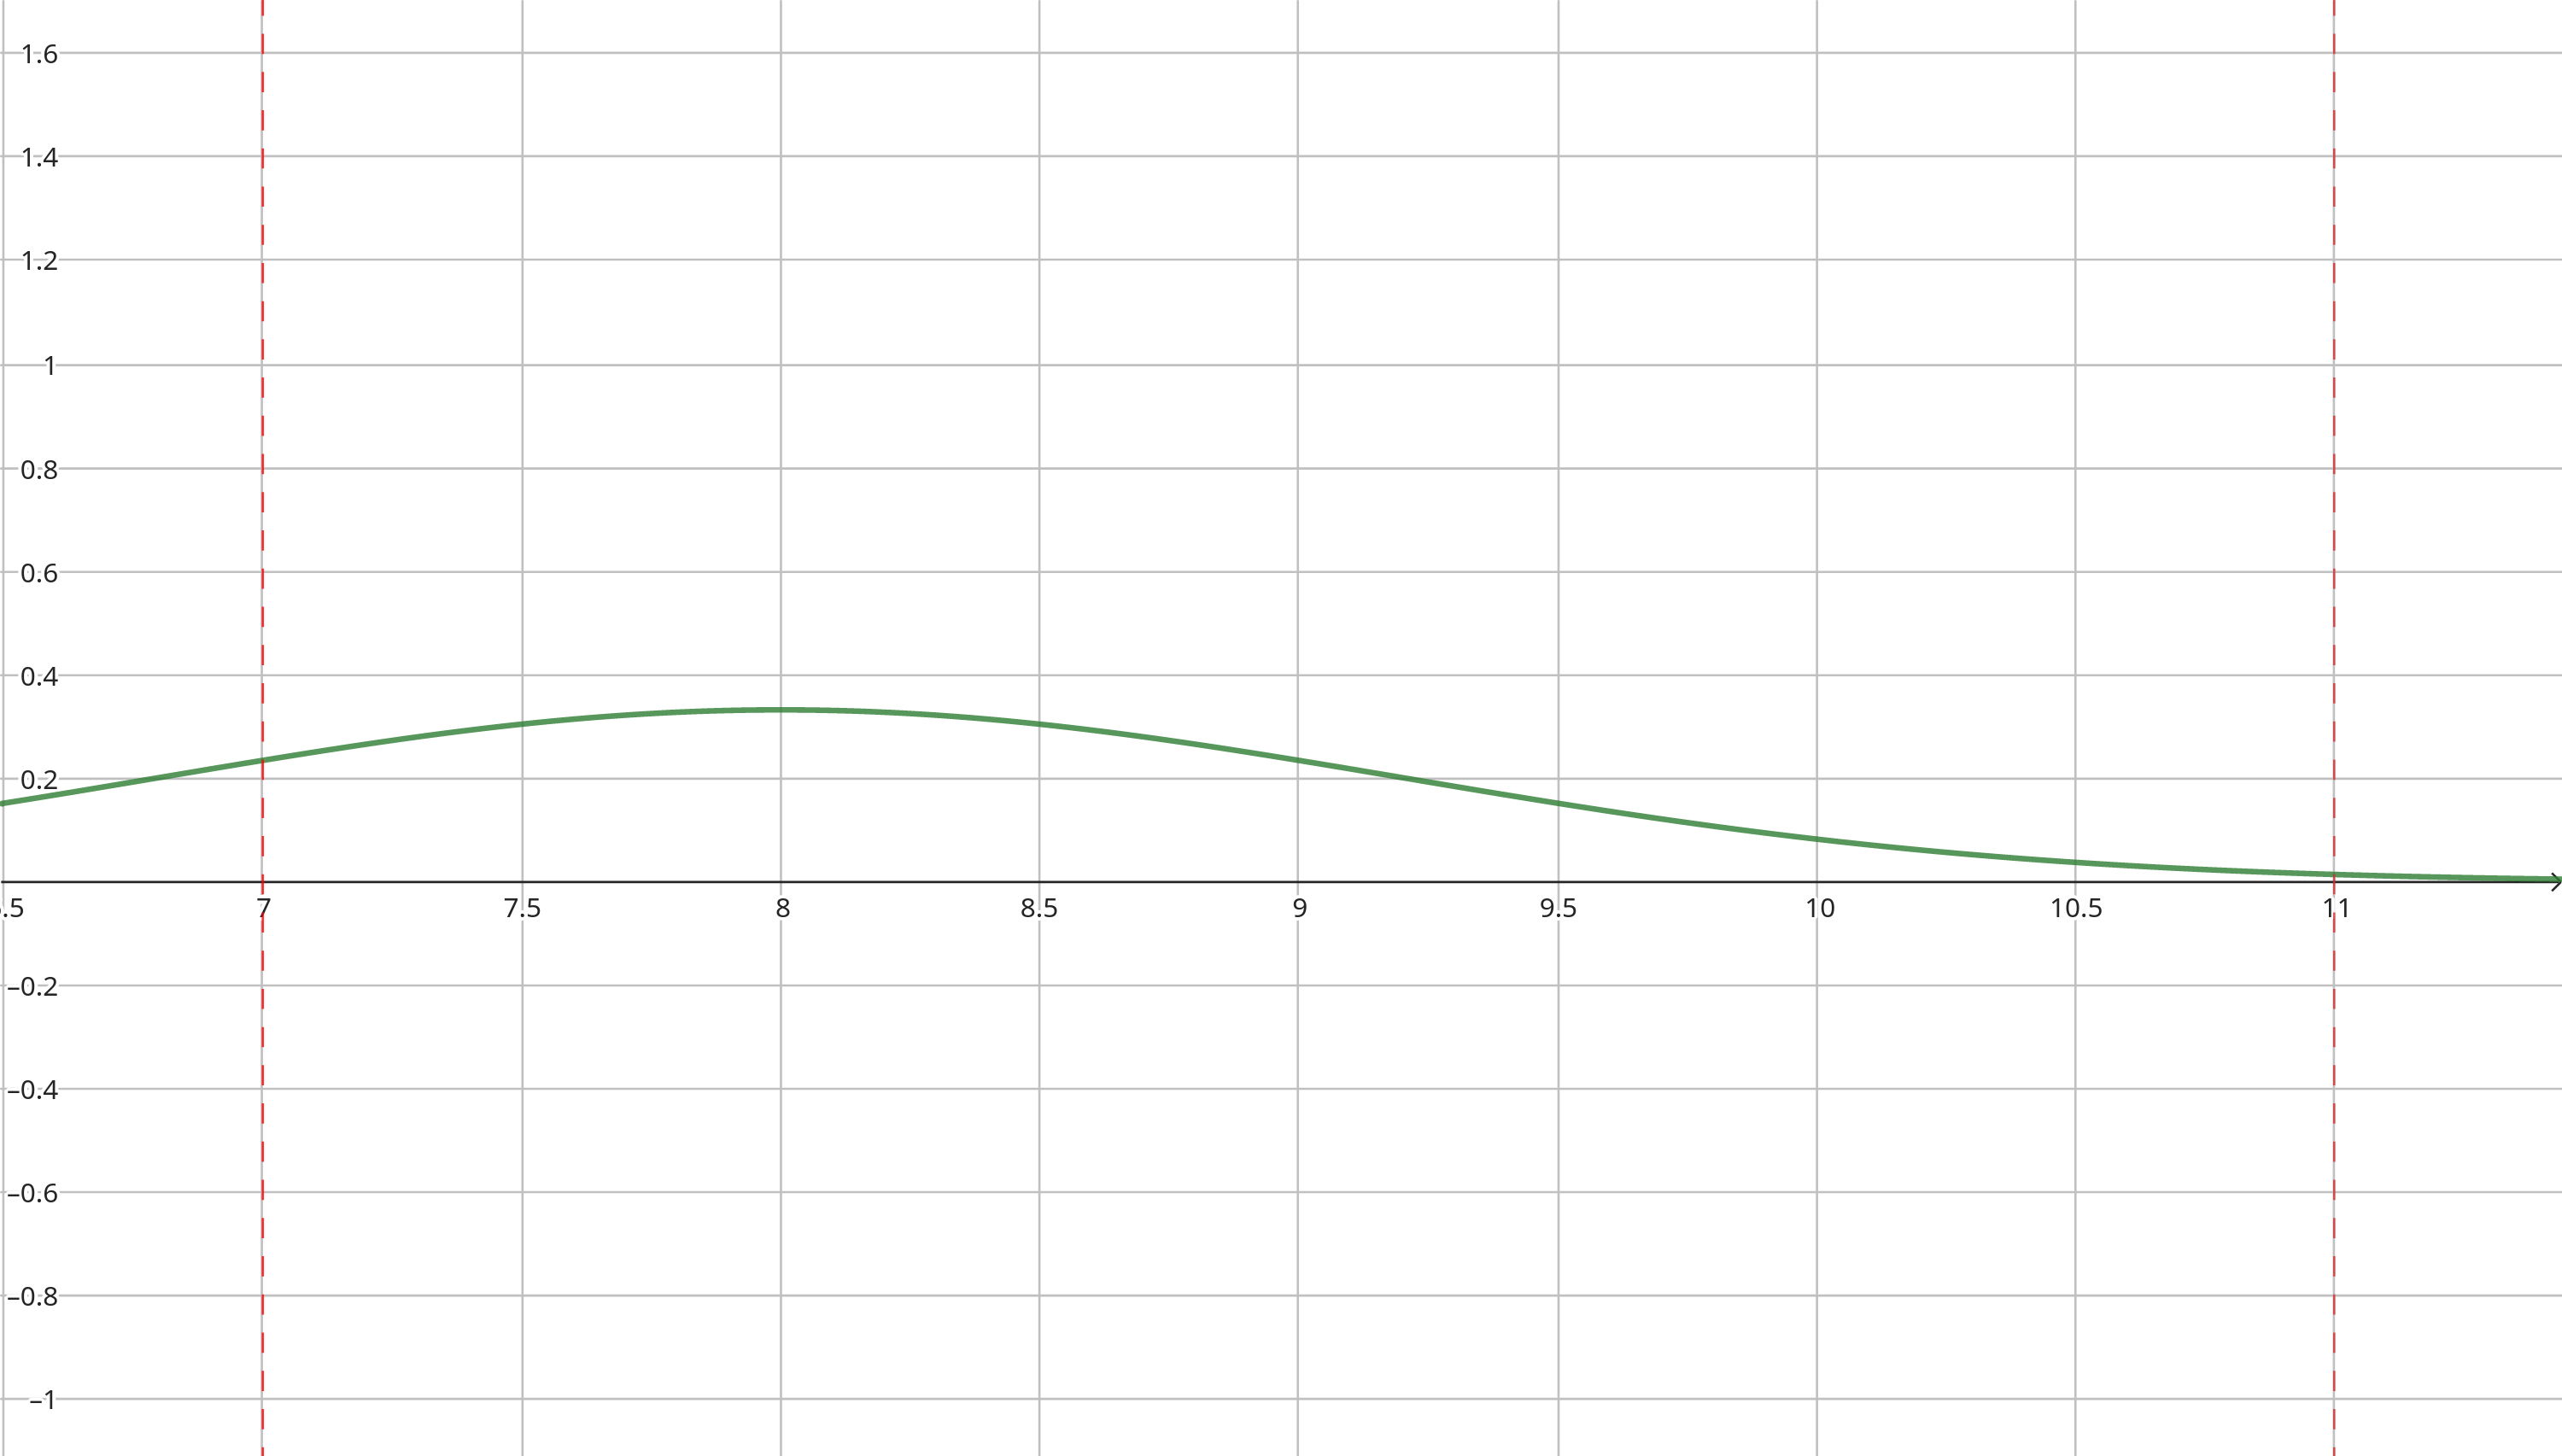
\includegraphics[width=0.7\textwidth]{7-11-gaussian}
\bigskip

\textit{Fascia oraria: 07:00 $\rightarrow$ 11:00}
\[ \mu = 8;\ \sigma = 1.2 \]
\end{figure}

\target{distribuzione gaussiana 11-15}
\begin{figure}[H]
\centering 
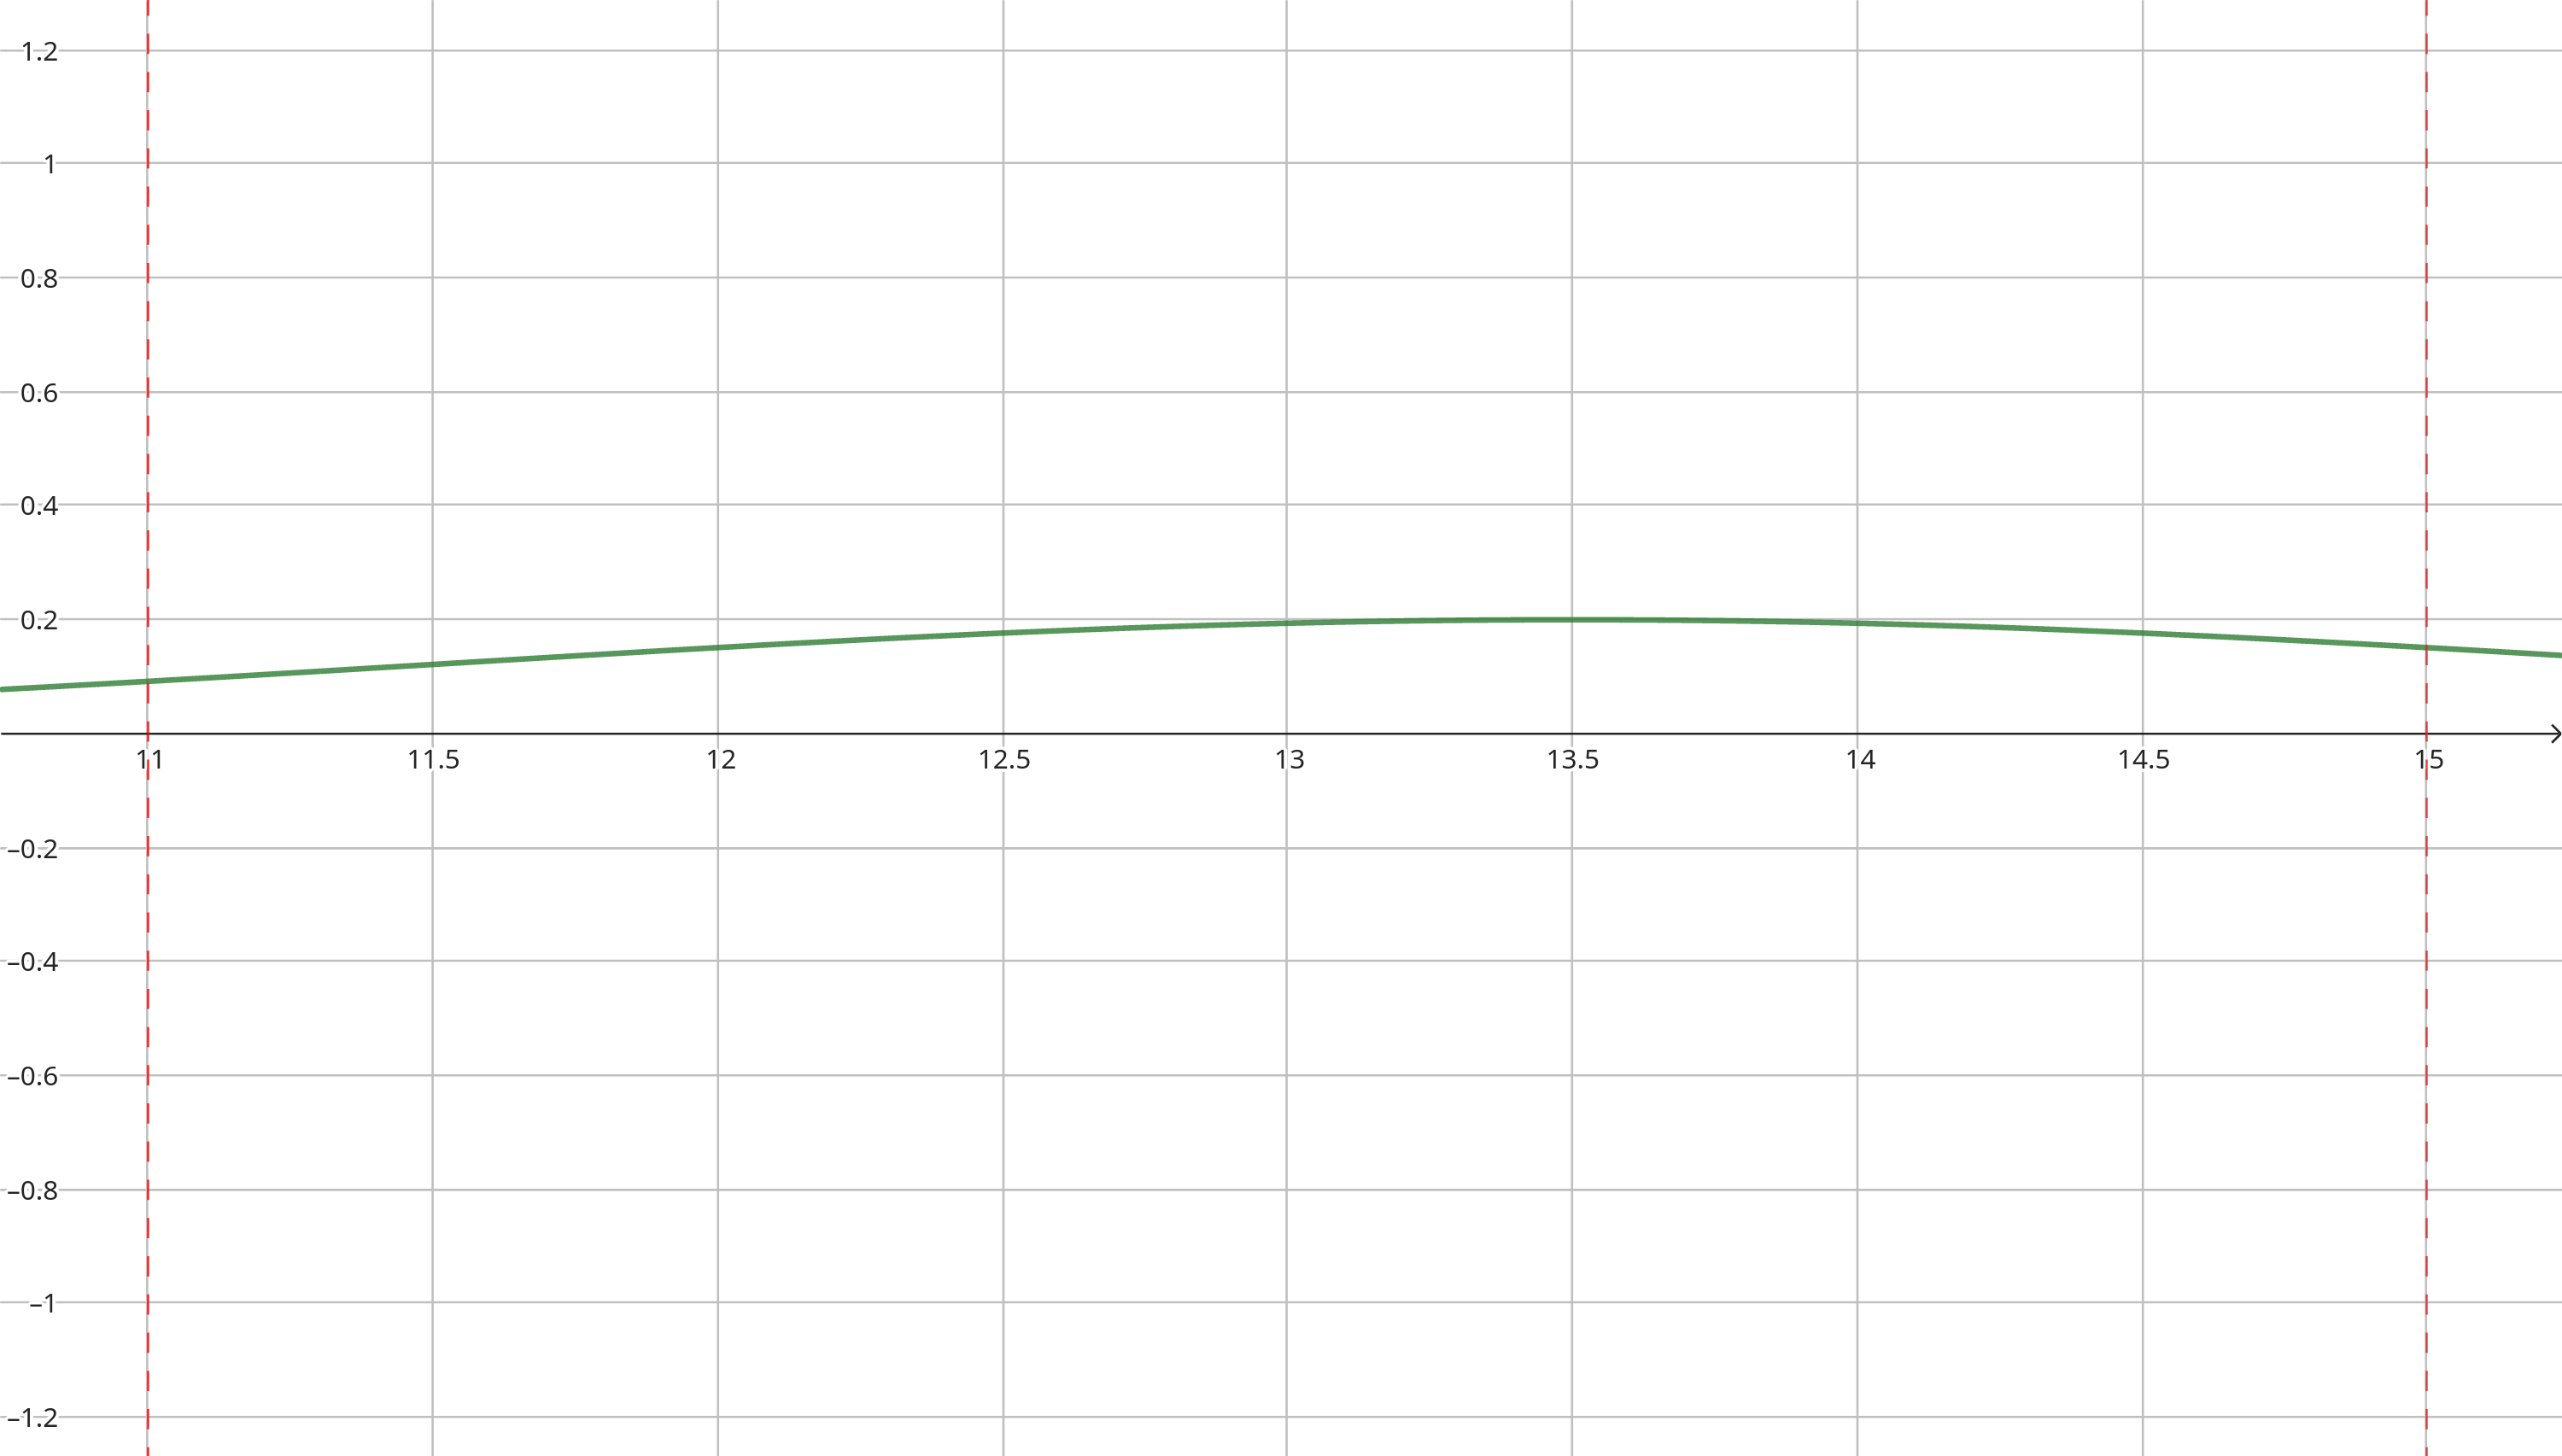
\includegraphics[width=0.7\textwidth]{11-15-gaussian}\bigskip

\textit{Fascia oraria: 11:00 $\rightarrow$ 15:00}
\[ \mu = 13.5;\ \sigma = 2 \]
\end{figure}

\target{distribuzione gaussiana 18-19}
\begin{figure}[H]
\centering 
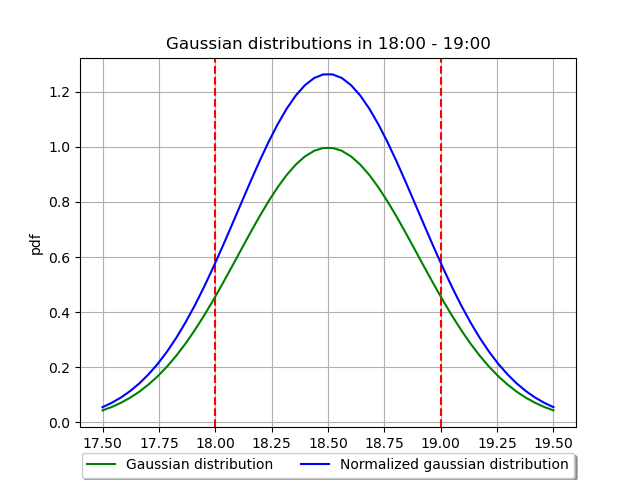
\includegraphics[width=0.7\textwidth]{18-19-gaussian}\bigskip

\textit{Fascia oraria: 18:00 $\rightarrow$ 19:00}
\[ \mu = 18.5;\ \sigma = 0.4 \]
\end{figure}

\target{distribuzione gaussiana 19-23}
\begin{figure}[H]
\centering 
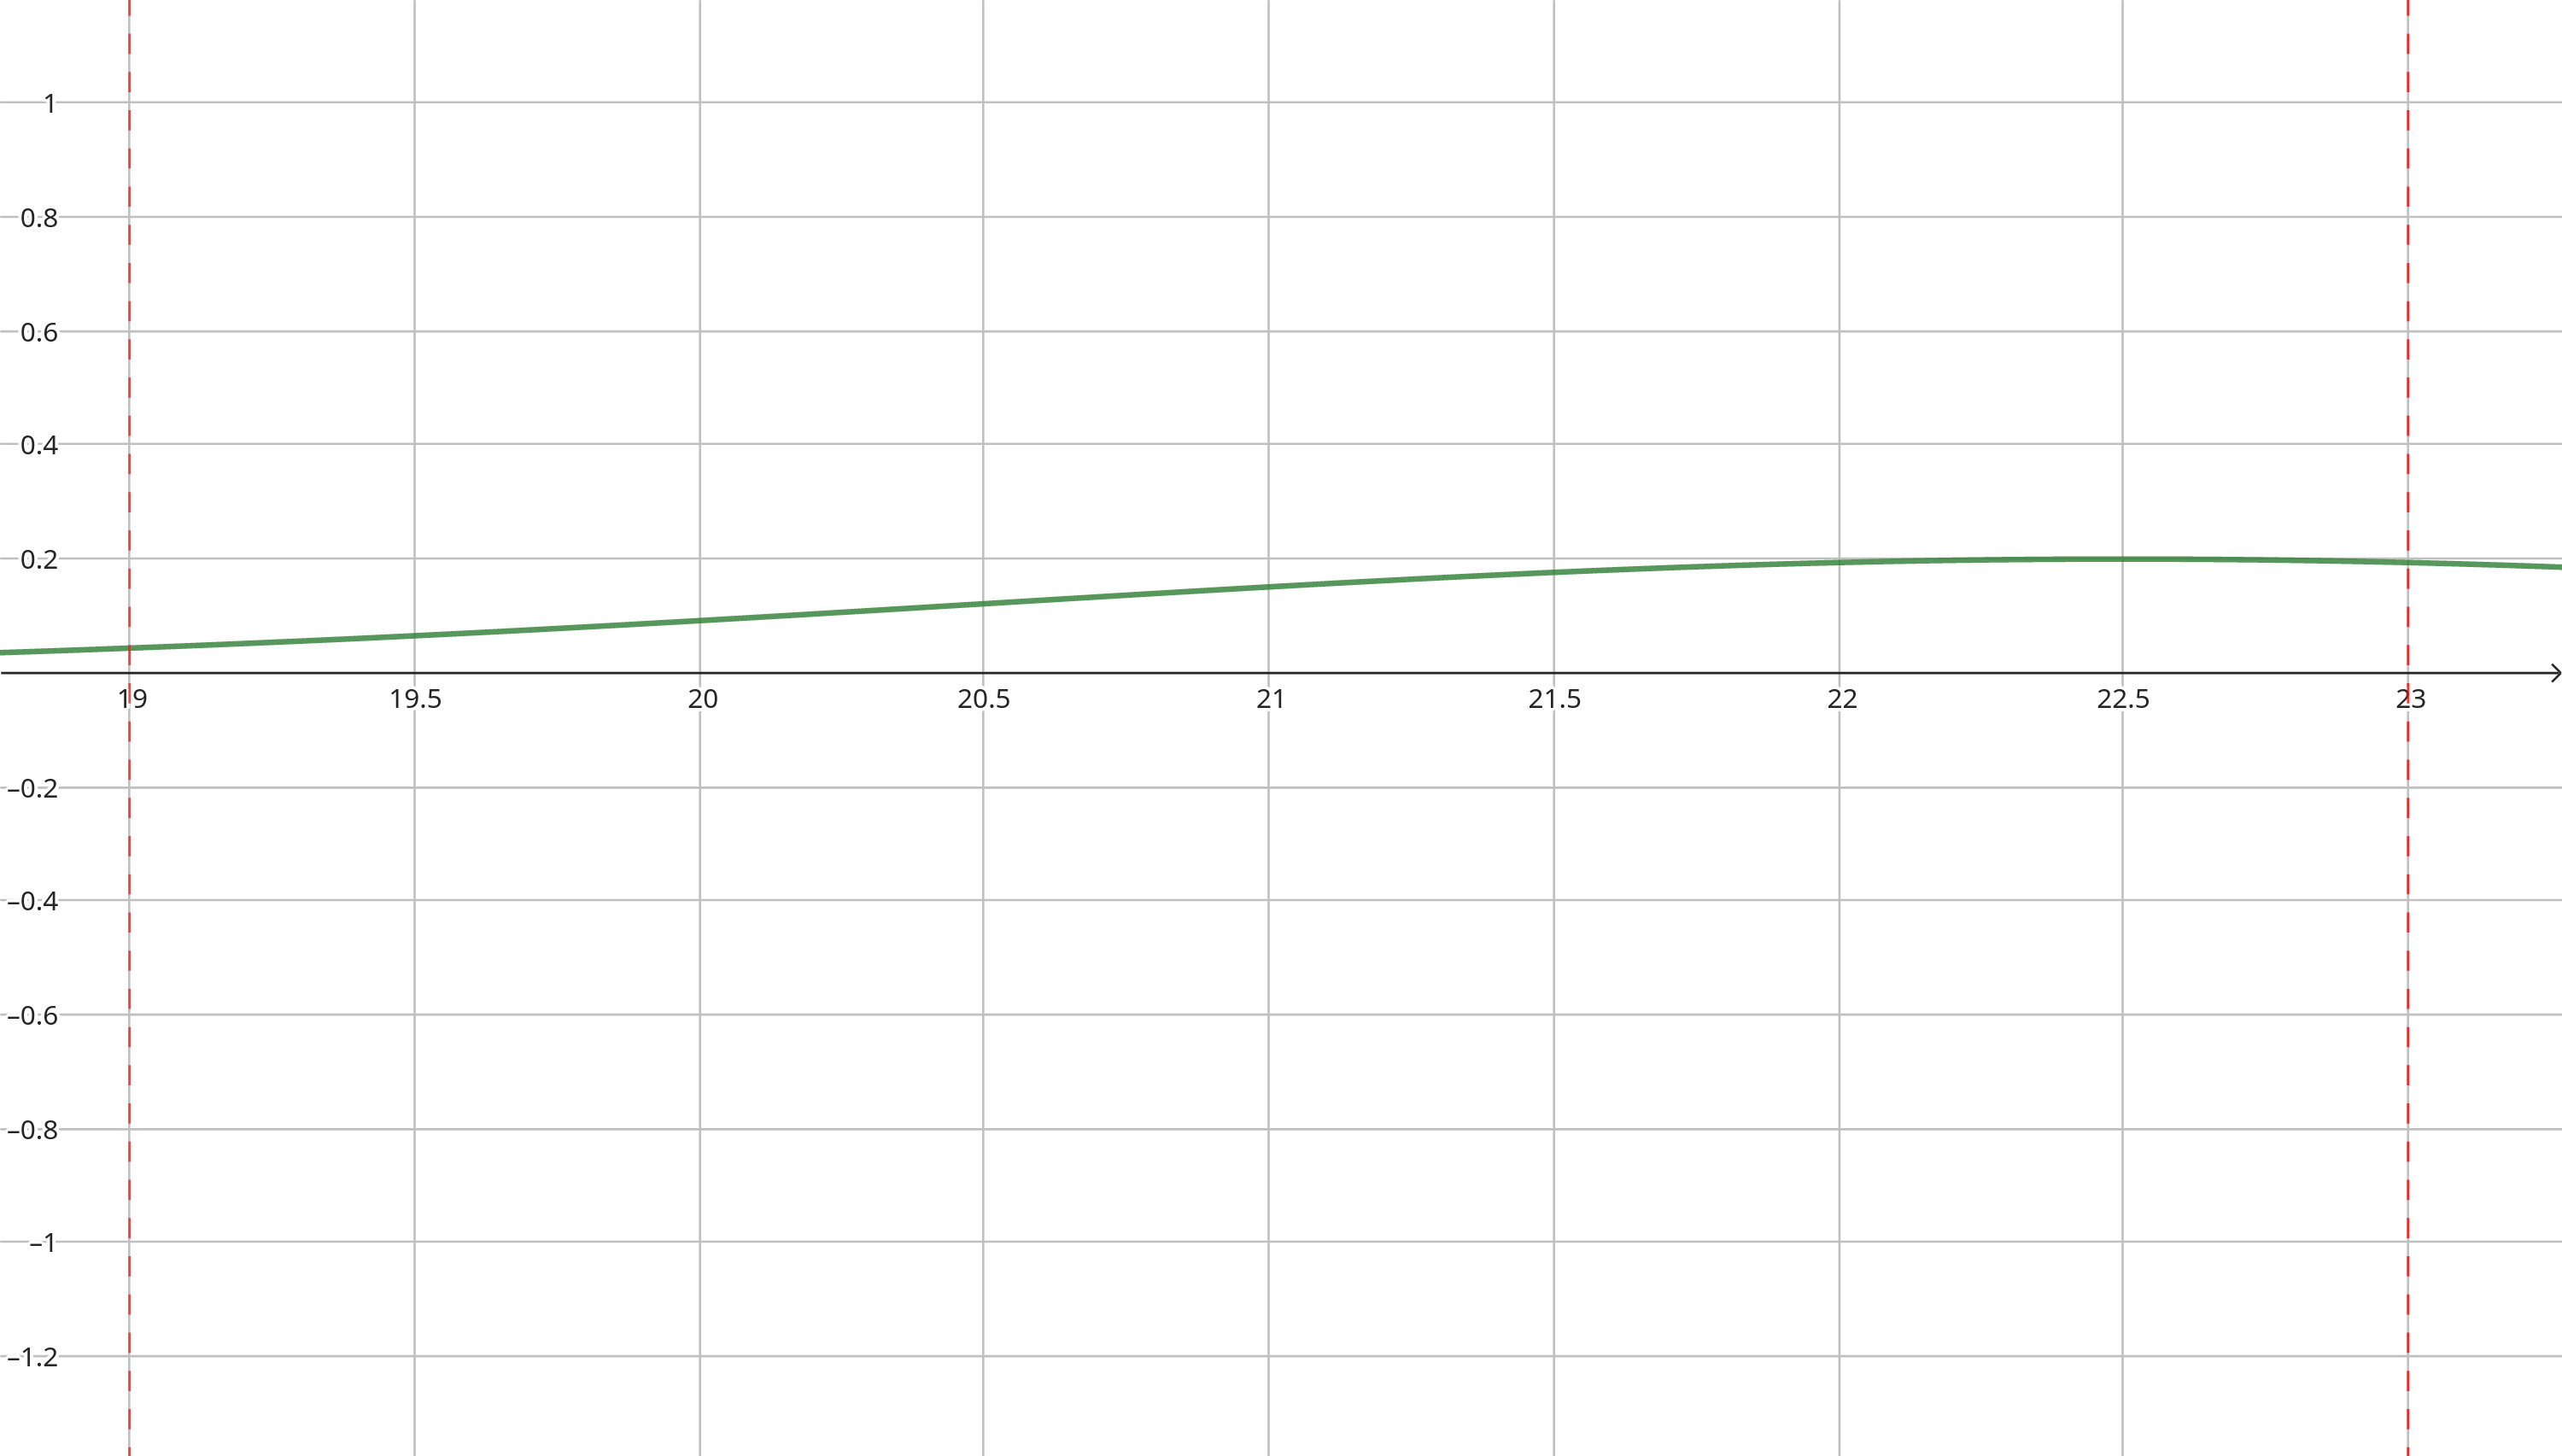
\includegraphics[width=0.7\textwidth]{19-23-gaussian}\bigskip

\textit{Fascia oraria: 19:00 $\rightarrow$ 23:00, bar}
\[ \mu = 22.5;\ \sigma = 2 \]
\end{figure}

\target{distribuzione gaussiana P}
\begin{figure}[H]
\centering 
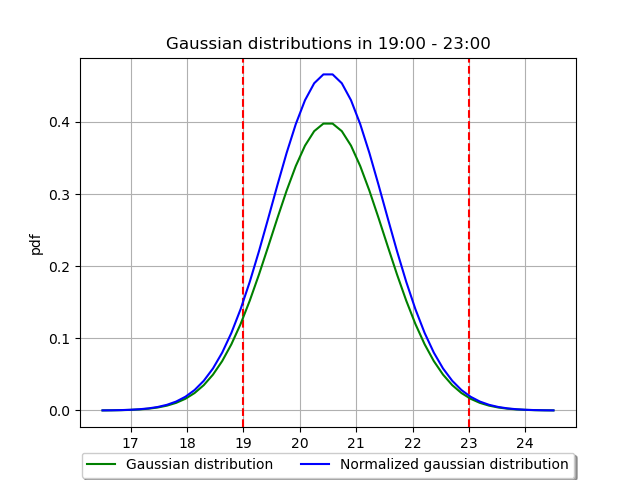
\includegraphics[width=0.7\textwidth]{19-23-gaussian-pizza}\bigskip

\textit{Fascia oraria: 19:00 $\rightarrow$ 23:00, pizzeria}
\[ \mu = 20.5;\ \sigma = 1 \]
\end{figure}

\target{distribuzione gaussiana 23-26}
\begin{figure}[H]
\centering 
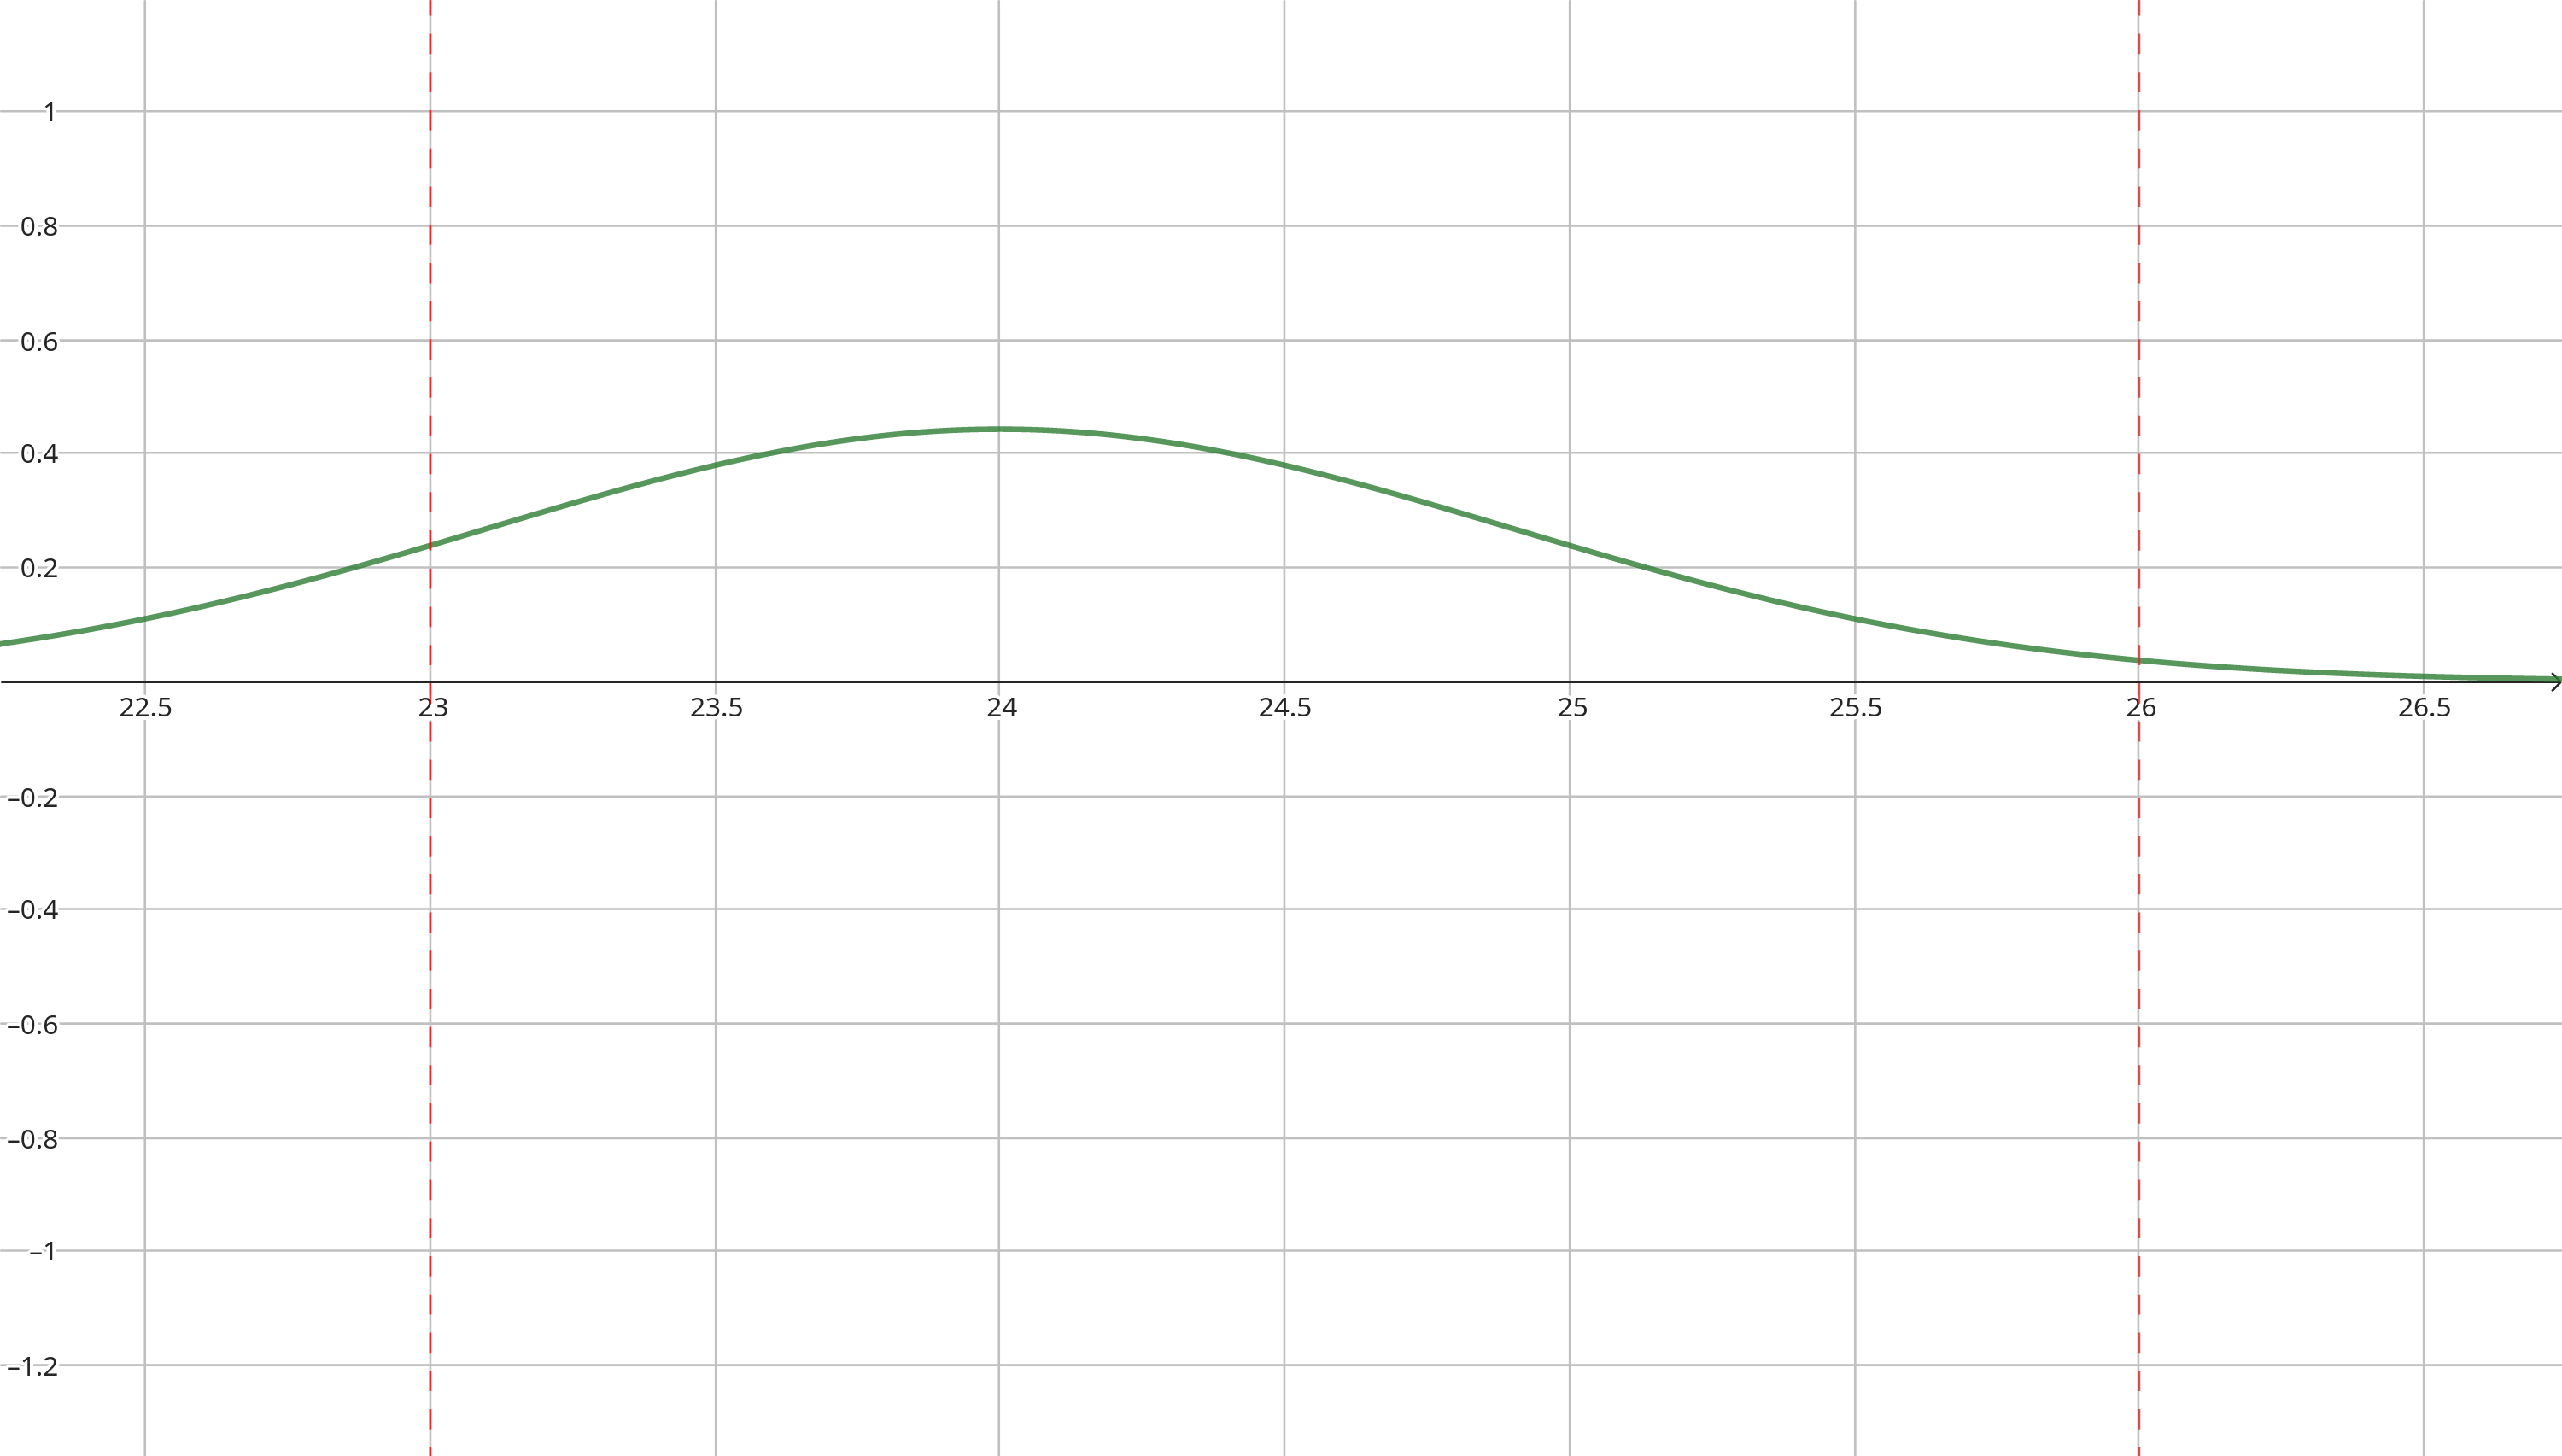
\includegraphics[width=0.7\textwidth]{23-02-gaussian}\bigskip

\textit{Fascia oraria: 23:00 $\rightarrow$ 02:00}
\[ \mu = 24;\ \sigma = 0.9 \]
\end{figure}

%__________________________________________


\subsection{Interarrivi}
\subsubsection{Week - orizzonte infinito}
\target{interarrivo infinito week slot 0}
\paragraph{Slot 0}
\subparagraph*{}
\begin{figure}[H]
\centering 
\includegraphics[width=0.8\textwidth]{/infinite/slot_0/avgInterarrivals/week_B_0}
\centering \textit{}
\end{figure}

\target{interarrivo infinito week slot 1}
\paragraph{Slot 1}
\subparagraph*{}
\begin{figure}[H]
\centering 
\includegraphics[width=0.8\textwidth]{/infinite/slot_1/avgInterarrivals/week_B_1}
\centering \textit{}
\end{figure}

\target{interarrivo infinito week slot 3}
\paragraph{Slot 3}
\subparagraph*{}
\begin{figure}[H]
\centering 
\includegraphics[width=0.8\textwidth]{/infinite/slot_3/avgInterarrivals/week_B_3}
\centering \textit{}
\end{figure}

\target{interarrivo infinito week slot 4}
\paragraph{Slot 4}
\subparagraph*{}
\begin{figure}[H]
\centering 
\includegraphics[width=0.8\textwidth]{/infinite/slot_4/avgInterarrivals/week_B_4}
\centering \textit{}
\end{figure}

\target{interarrivo infinito week slot 5}
\paragraph{Slot 5}
\subparagraph*{}
\begin{figure}[H]
\centering 
\includegraphics[width=0.8\textwidth]{/infinite/slot_5/avgInterarrivals/week_B_5}
\centering \textit{}
\end{figure}

\paragraph{P}
\target{interarrivo infinito week P}
\subparagraph*{}
\begin{figure}[H]
\centering 
\includegraphics[width=0.8\textwidth]{/infinite/slot_4/avgInterarrivals/week_P_4}
\centering \textit{}
\end{figure}


\subsubsection{Weekend - orizzonte infinito}
\target{interarrivo infinito weekend slot 0}
\paragraph{Slot 0}
\subparagraph*{}
\begin{figure}[H]
\centering 
\includegraphics[width=0.8\textwidth]{/infinite/slot_0/avgInterarrivals/weekend_B_0}
\centering \textit{}
\end{figure}

\paragraph{Slot 1}
\target{interarrivo infinito weekend slot 1}
\subparagraph*{}
\begin{figure}[H]
\centering 
\includegraphics[width=0.8\textwidth]{/infinite/slot_1/avgInterarrivals/weekend_B_1}
\centering \textit{}
\end{figure}

\paragraph{Slot 3}
\target{interarrivo infinito weekend slot 3}
\subparagraph*{}
\begin{figure}[H]
\centering 
\includegraphics[width=0.8\textwidth]{/infinite/slot_3/avgInterarrivals/weekend_B_3}
\centering \textit{}
\end{figure}

\paragraph{Slot 4}
\target{interarrivo infinito weekend slot 4}
\subparagraph*{}
\begin{figure}[H]
\centering 
\includegraphics[width=0.8\textwidth]{/infinite/slot_4/avgInterarrivals/weekend_B_4}
\centering \textit{}
\end{figure}

\paragraph{Slot 5}
\target{interarrivo infinito weekend slot 5}
\subparagraph*{}
\begin{figure}[H]
\centering 
\includegraphics[width=0.8\textwidth]{/infinite/slot_5/avgInterarrivals/weekend_B_5}
\centering \textit{}
\end{figure}

\paragraph{P}
\target{interarrivo infinito weekend P}
\subparagraph*{}
\begin{figure}[H]
\centering 
\includegraphics[width=0.8\textwidth]{/infinite/slot_4/avgInterarrivals/weekend_P_4}
\centering \textit{}
\end{figure}
%__________________________________________



\subsection{Attesa}
\subsubsection{Week - orizzonte infinito}
\target{attesa infinita week slot 0}
\paragraph{Slot 0}
\subparagraph*{}
\begin{figure}[H]
\centering 
\includegraphics[width=0.8\textwidth]{/infinite/slot_0/avgWaits/week_B_0}
\centering \textit{}
\end{figure}

\target{attesa infinita week slot 1}
\paragraph{Slot 1}
\subparagraph*{}
\begin{figure}[H]
\centering 
\includegraphics[width=0.8\textwidth]{/infinite/slot_1/avgWaits/week_B_1}
\centering \textit{}
\end{figure}

\target{attesa infinita week slot 3}
\paragraph{Slot 3}
\subparagraph*{}
\begin{figure}[H]
\centering 
\includegraphics[width=0.8\textwidth]{/infinite/slot_3/avgWaits/week_B_3}
\centering \textit{}
\end{figure}

\target{attesa infinita week slot 4}
\paragraph{Slot 4}
\subparagraph*{}
\begin{figure}[H]
\centering 
\includegraphics[width=0.8\textwidth]{/infinite/slot_4/avgWaits/week_B_4}
\centering \textit{}
\end{figure}

\target{attesa infinita week slot 5}
\paragraph{Slot 5}
\subparagraph*{}
\begin{figure}[H]
\centering 
\includegraphics[width=0.8\textwidth]{/infinite/slot_5/avgWaits/week_B_5}
\centering \textit{}
\end{figure}

\paragraph{P}
\target{attesa infinita week P}
\subparagraph*{}
\begin{figure}[H]
\centering 
\includegraphics[width=0.8\textwidth]{/infinite/slot_4/avgWaits/week_P_4}
\centering \textit{}
\end{figure}


\subsubsection{Weekend - orizzonte infinito}
\target{attesa infinita weekend slot 0}
\paragraph{Slot 0}
\subparagraph*{}
\begin{figure}[H]
\centering 
\includegraphics[width=0.8\textwidth]{/infinite/slot_0/avgWaits/weekend_B_0}
\centering \textit{}
\end{figure}

\target{attesa infinita weekend slot 1}
\paragraph{Slot 1}
\subparagraph*{}
\begin{figure}[H]
\centering 
\includegraphics[width=0.8\textwidth]{/infinite/slot_1/avgWaits/weekend_B_1}
\centering \textit{}
\end{figure}

\target{attesa infinita weekend slot 3}
\paragraph{Slot 3}
\subparagraph*{}
\begin{figure}[H]
\centering 
\includegraphics[width=0.8\textwidth]{/infinite/slot_3/avgWaits/weekend_B_3}
\centering \textit{}
\end{figure}

\target{attesa infinita weekend slot 4}
\paragraph{Slot 4}
\subparagraph*{}
\begin{figure}[H]
\centering 
\includegraphics[width=0.8\textwidth]{/infinite/slot_4/avgWaits/weekend_B_4}
\centering \textit{}
\end{figure}

\target{attesa infinita weekend slot 5}
\paragraph{Slot 5}
\subparagraph*{}
\begin{figure}[H]
\centering 
\includegraphics[width=0.8\textwidth]{/infinite/slot_5/avgWaits/weekend_B_5}
\centering \textit{}
\end{figure}

\paragraph{P}
\target{attesa infinita weekend P}
\subparagraph*{}
\begin{figure}[H]
\centering 
\includegraphics[width=0.8\textwidth]{/infinite/slot_4/avgWaits/weekend_P_4}
\centering \textit{}
\end{figure}


\subsubsection{Week - orizzonte finito}
\target{attesa finita week B no gau}
\paragraph{Tipo B - no gaussian factor}
\subparagraph*{}
\begin{figure}[H]
\centering 
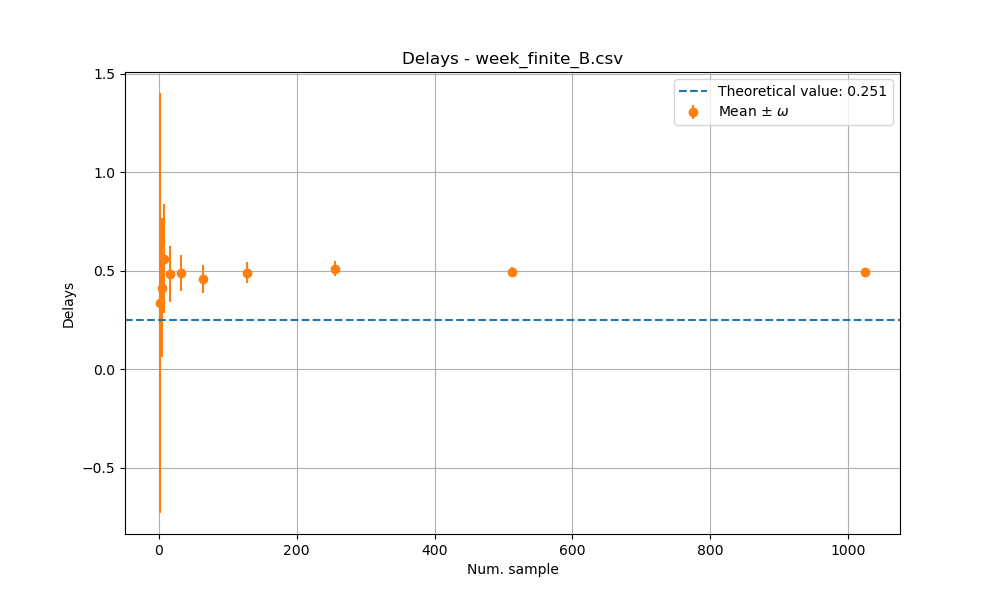
\includegraphics[width=0.8\textwidth]{/finite/avgWaits/week_B}
\centering \textit{}
\end{figure}

\target{attesa finita week P no gau}
\paragraph{Tipo P - no gaussian factor}
\subparagraph*{}
\begin{figure}[H]
\centering 
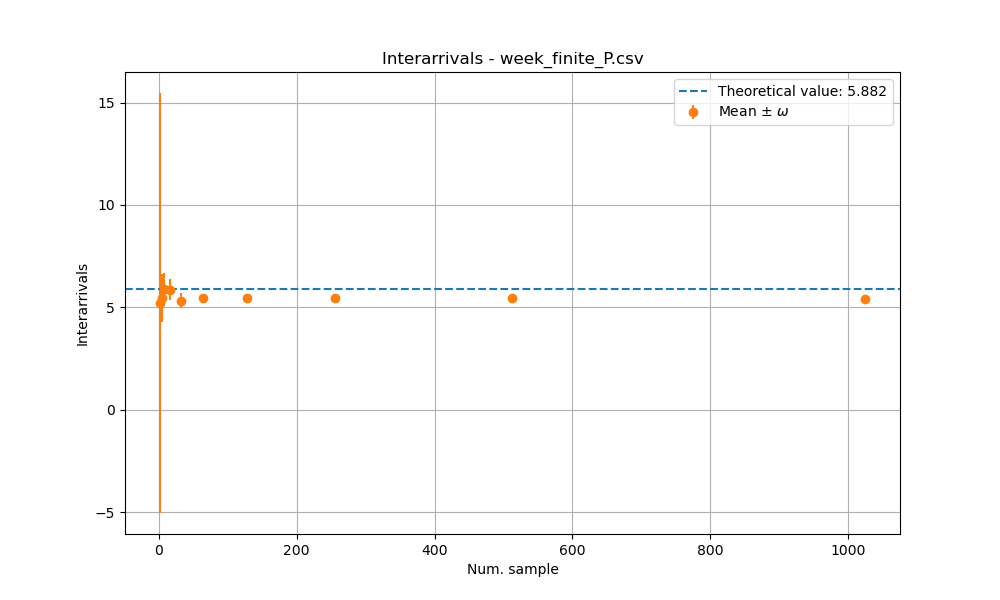
\includegraphics[width=0.8\textwidth]{/finite/avgWaits/week_P}
\centering \textit{}
\end{figure}

\target{attesa finita week B gau}
\paragraph{Tipo B - gaussian factor}
\subparagraph*{}
\begin{figure}[H]
\centering 
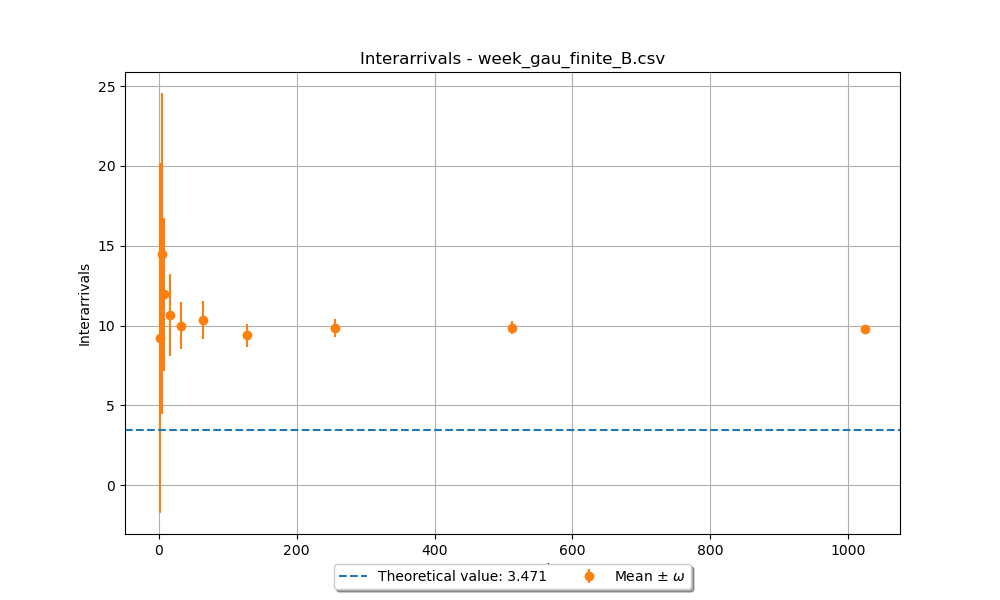
\includegraphics[width=0.8\textwidth]{/finite/avgWaits/week_B_gau}
\centering \textit{}
\end{figure}

\target{attesa finita week P gau}
\paragraph{Tipo P - gaussian factor}
\subparagraph*{}
\begin{figure}[H]
\centering 
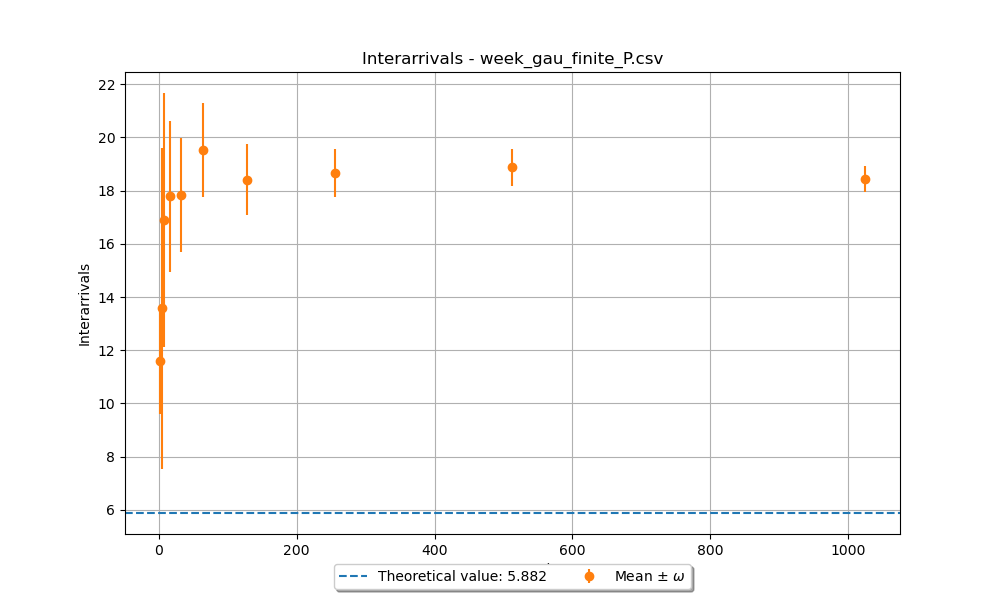
\includegraphics[width=0.8\textwidth]{/finite/avgWaits/week_P_gau}
\centering \textit{}
\end{figure}



\subsubsection{Weekend - orizzonte finito}
\target{attesa finita weekend B no gau}
\paragraph{Tipo B}
\subparagraph*{}
\begin{figure}[H]
\centering 
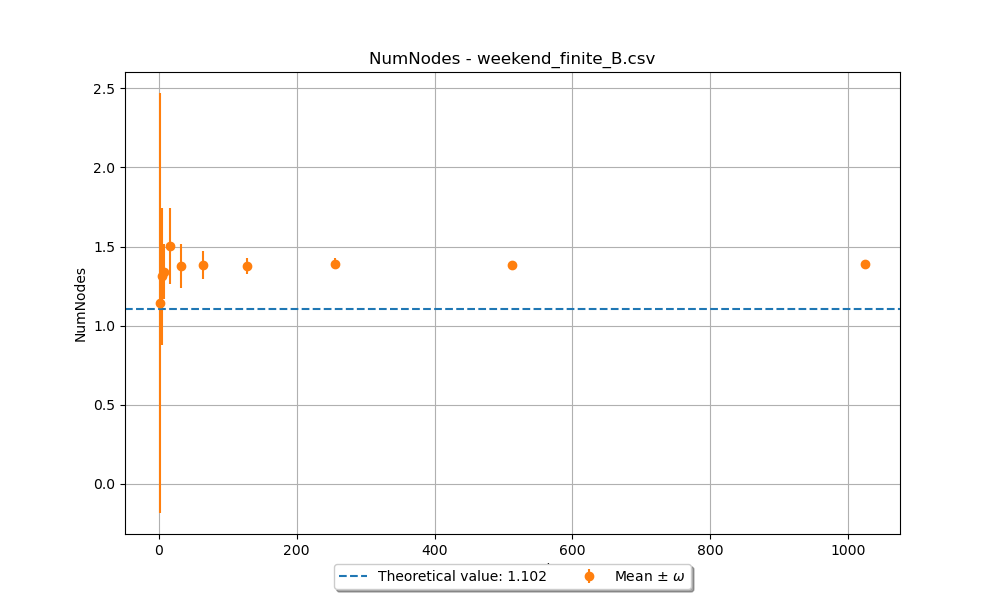
\includegraphics[width=0.8\textwidth]{/finite/avgWaits/weekend_B}
\centering \textit{}
\end{figure}

\target{attesa finita weekend P no gau}
\paragraph{Tipo P}
\subparagraph*{}
\begin{figure}[H]
\centering 
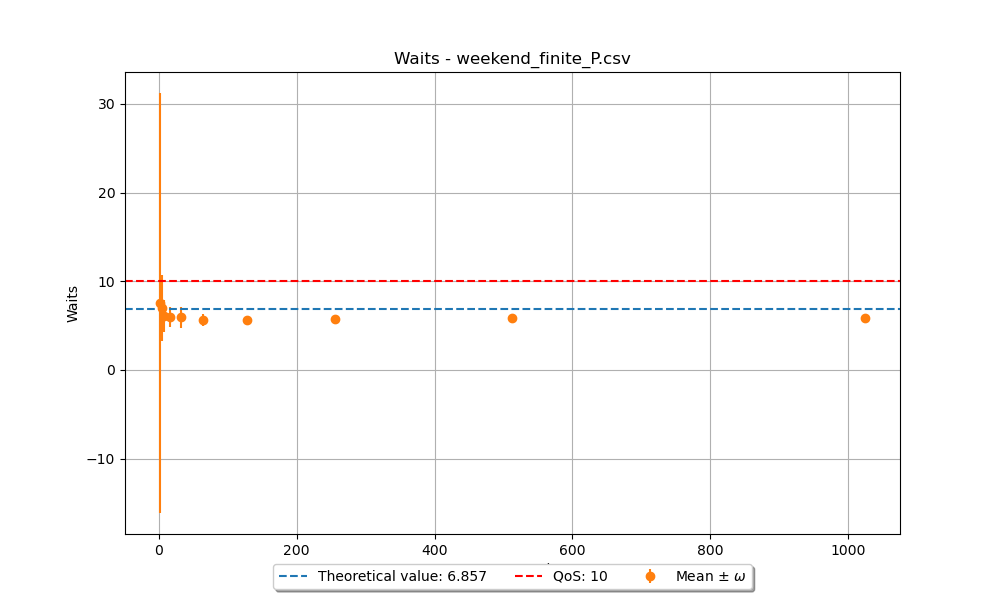
\includegraphics[width=0.8\textwidth]{/finite/avgWaits/weekend_P}
\centering \textit{}
\end{figure}

\target{attesa finita weekend B gau}
\paragraph{Tipo B - gaussian factor}
\subparagraph*{}
\begin{figure}[H]
\centering 
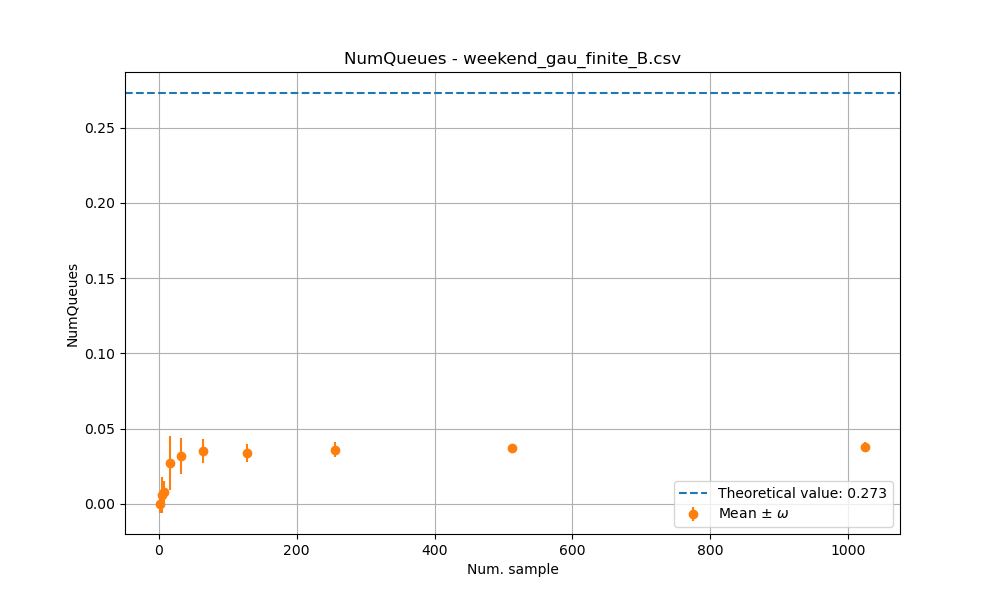
\includegraphics[width=0.8\textwidth]{/finite/avgWaits/weekend_B_gau}
\centering \textit{}
\end{figure}

\target{attesa finita weekend P gau}
\paragraph{Tipo P - gaussian factor}
\subparagraph*{}
\begin{figure}[H]
\centering 
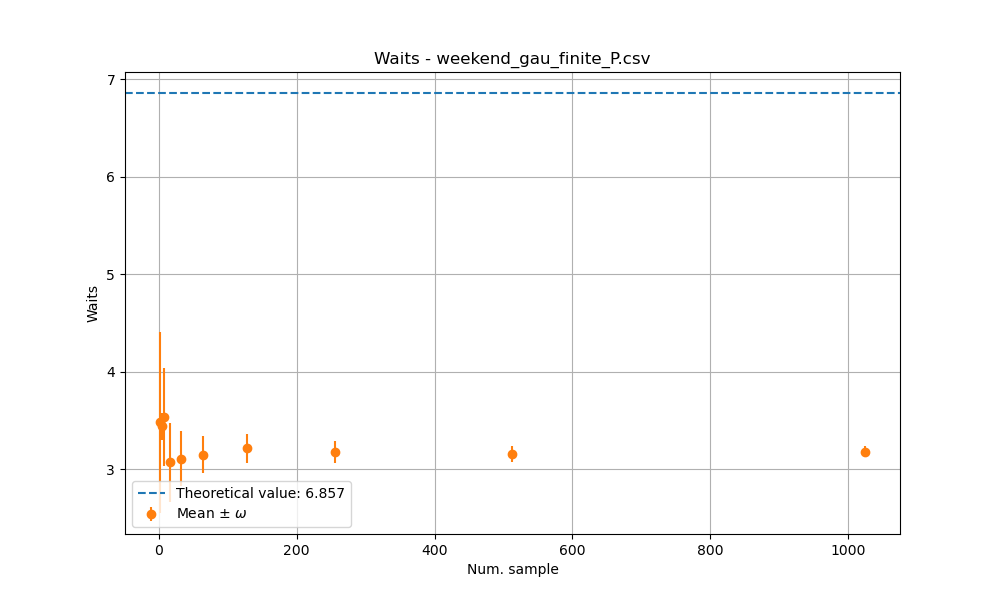
\includegraphics[width=0.8\textwidth]{/finite/avgWaits/weekend_P_gau}
\centering \textit{}
\end{figure}


%__________________________________________

\subsection{Popolazione nel centro}
\subsubsection{Week - orizzonte infinito}
\target{centro infinito week slot 0}
\paragraph{Slot 0}
\subparagraph*{}
\begin{figure}[H]
\centering 
\includegraphics[width=0.8\textwidth]{/infinite/slot_0/avgNumNodes/week_B_0}
\centering \textit{}
\end{figure}

\target{centro infinito week slot 1}
\paragraph{Slot 1}
\subparagraph*{}
\begin{figure}[H]
\centering 
\includegraphics[width=0.8\textwidth]{/infinite/slot_1/avgNumNodes/week_B_1}
\centering \textit{}
\end{figure}

\target{centro infinito week slot 3}
\paragraph{Slot 3}
\subparagraph*{}
\begin{figure}[H]
\centering 
\includegraphics[width=0.8\textwidth]{/infinite/slot_3/avgNumNodes/week_B_3}
\centering \textit{}
\end{figure}

\target{centro infinito week slot 4}
\paragraph{Slot 4}
\subparagraph*{}
\begin{figure}[H]
\centering 
\includegraphics[width=0.8\textwidth]{/infinite/slot_4/avgNumNodes/week_B_4}
\centering \textit{}
\end{figure}

\target{centro infinito week slot 5}
\paragraph{Slot 5}
\subparagraph*{}
\begin{figure}[H]
\centering 
\includegraphics[width=0.8\textwidth]{/infinite/slot_5/avgNumNodes/week_B_5}
\centering \textit{}
\end{figure}

\paragraph{P}
\target{centro infinito week P}
\subparagraph*{}
\begin{figure}[H]
\centering 
\includegraphics[width=0.8\textwidth]{/infinite/slot_4/avgNumNodes/week_P_4}
\centering \textit{}
\end{figure}


\subsubsection{Weekend - orizzonte infinito}
\target{centro infinito weekend slot 0}
\paragraph{Slot 0}
\subparagraph*{}
\begin{figure}[H]
\centering 
\includegraphics[width=0.8\textwidth]{/infinite/slot_0/avgNumNodes/weekend_B_0}
\centering \textit{}
\end{figure}

\target{centro infinito weekend slot 1}
\paragraph{Slot 1}
\subparagraph*{}
\begin{figure}[H]
\centering 
\includegraphics[width=0.8\textwidth]{/infinite/slot_1/avgNumNodes/weekend_B_1}
\centering \textit{}
\end{figure}

\target{centro infinito weekend slot 3}
\paragraph{Slot 3}
\subparagraph*{}
\begin{figure}[H]
\centering 
\includegraphics[width=0.8\textwidth]{/infinite/slot_3/avgNumNodes/weekend_B_3}
\centering \textit{}
\end{figure}

\target{centro infinito weekend slot 4}
\paragraph{Slot 4}
\subparagraph*{}
\begin{figure}[H]
\centering 
\includegraphics[width=0.8\textwidth]{/infinite/slot_4/avgNumNodes/weekend_B_4}
\centering \textit{}
\end{figure}

\target{centro infinito weekend slot 5}
\paragraph{Slot 5}
\subparagraph*{}
\begin{figure}[H]
\centering 
\includegraphics[width=0.8\textwidth]{/infinite/slot_5/avgNumNodes/weekend_B_5}
\centering \textit{}
\end{figure}

\paragraph{P}
\target{centro infinito weekend P}
\subparagraph*{}
\begin{figure}[H]
\centering 
\includegraphics[width=0.8\textwidth]{/infinite/slot_4/avgNumNodes/weekend_P_4}
\centering \textit{}
\end{figure}

%__________________________________________


\subsection{Ritardo}
\subsubsection{Week - orizzonte infinito}
\target{ritardo infinito week slot 0}
\paragraph{Slot 0}
\subparagraph*{}
\begin{figure}[H]
\centering 
\includegraphics[width=0.8\textwidth]{/infinite/slot_0/avgDelays/week_B_0}
\centering \textit{}
\end{figure}

\target{ritardo infinito week slot 1}
\paragraph{Slot 1}
\subparagraph*{}
\begin{figure}[H]
\centering 
\includegraphics[width=0.8\textwidth]{/infinite/slot_1/avgDelays/week_B_1}
\centering \textit{}
\end{figure}

\target{ritardo infinito week slot 3}
\paragraph{Slot 3}
\subparagraph*{}
\begin{figure}[H]
\centering 
\includegraphics[width=0.8\textwidth]{/infinite/slot_3/avgDelays/week_B_3}
\centering \textit{}
\end{figure}

\target{ritardo infinito week slot 4}
\paragraph{Slot 4}
\subparagraph*{}
\begin{figure}[H]
\centering 
\includegraphics[width=0.8\textwidth]{/infinite/slot_4/avgDelays/week_B_4}
\centering \textit{}
\end{figure}

\target{ritardo infinito week slot 5}
\paragraph{Slot 5}
\subparagraph*{}
\begin{figure}[H]
\centering 
\includegraphics[width=0.8\textwidth]{/infinite/slot_5/avgDelays/week_B_5}
\centering \textit{}
\end{figure}

\paragraph{P}
\target{ritardo infinito week P}
\subparagraph*{}
\begin{figure}[H]
\centering 
\includegraphics[width=0.8\textwidth]{/infinite/slot_4/avgDelays/week_P_4}
\centering \textit{}
\end{figure}


\subsubsection{Weekend - orizzonte infinito}
\target{ritardo infinito weekend slot 0}
\paragraph{Slot 0}
\subparagraph*{}
\begin{figure}[H]
\centering 
\includegraphics[width=0.8\textwidth]{/infinite/slot_0/avgDelays/weekend_B_0}
\centering \textit{}
\end{figure}

\target{ritardo infinito weekend slot 1}
\paragraph{Slot 1}
\subparagraph*{}
\begin{figure}[H]
\centering 
\includegraphics[width=0.8\textwidth]{/infinite/slot_1/avgDelays/weekend_B_1}
\centering \textit{}
\end{figure}

\target{ritardo infinito weekend slot 3}
\paragraph{Slot 3}
\subparagraph*{}
\begin{figure}[H]
\centering 
\includegraphics[width=0.8\textwidth]{/infinite/slot_3/avgDelays/weekend_B_3}
\centering \textit{}
\end{figure}

\target{ritardo infinito weekend slot 4}
\paragraph{Slot 4}
\subparagraph*{}
\begin{figure}[H]
\centering 
\includegraphics[width=0.8\textwidth]{/infinite/slot_4/avgDelays/weekend_B_4}
\centering \textit{}
\end{figure}

\paragraph{P}
\target{ritardo infinito weekend P}
\subparagraph*{}
\begin{figure}[H]
\centering 
\includegraphics[width=0.8\textwidth]{/infinite/slot_4/avgDelays/weekend_P_4}
\centering \textit{}
\end{figure}

\target{ritardo infinito weekend slot 5}
\paragraph{Slot 5}
\subparagraph*{}
\begin{figure}[H]
\centering 
\includegraphics[width=0.8\textwidth]{/infinite/slot_5/avgDelays/weekend_B_5}
\centering \textit{}
\end{figure}


%__________________________________________


\subsection{Popolazione in coda}
\subsubsection{Week - orizzonte infinito}
\target{coda infinita week slot 0}
\paragraph{Slot 0}
\subparagraph*{}
\begin{figure}[H]
\centering 
\includegraphics[width=0.8\textwidth]{/infinite/slot_0/avgNumQueues/week_B_0}
\centering \textit{}
\end{figure}

\target{coda infinita week slot 1}
\paragraph{Slot 1}
\subparagraph*{}
\begin{figure}[H]
\centering 
\includegraphics[width=0.8\textwidth]{/infinite/slot_1/avgNumQueues/week_B_1}
\centering \textit{}
\end{figure}

\target{coda infinita week slot 3}
\paragraph{Slot 3}
\subparagraph*{}
\begin{figure}[H]
\centering 
\includegraphics[width=0.8\textwidth]{/infinite/slot_3/avgNumQueues/week_B_3}
\centering \textit{}
\end{figure}

\target{coda infinita week slot 4}
\paragraph{Slot 4}
\subparagraph*{}
\begin{figure}[H]
\centering 
\includegraphics[width=0.8\textwidth]{/infinite/slot_4/avgNumQueues/week_B_4}
\centering \textit{}
\end{figure}

\target{coda infinita week slot 5}
\paragraph{Slot 5}
\subparagraph*{}
\begin{figure}[H]
\centering 
\includegraphics[width=0.8\textwidth]{/infinite/slot_5/avgNumQueues/week_B_5}
\centering \textit{}
\end{figure}

\paragraph{P}
\target{coda infinita week P}
\subparagraph*{}
\begin{figure}[H]
\centering 
\includegraphics[width=0.8\textwidth]{/infinite/slot_4/avgNumQueues/week_P_4}
\centering \textit{}
\end{figure}

\subsubsection{Weekend - orizzonte infinito}
\target{coda infinita weekend slot 0}
\paragraph{Slot 0}
\subparagraph*{}
\begin{figure}[H]
\centering 
\includegraphics[width=0.8\textwidth]{/infinite/slot_0/avgNumQueues/weekend_B_0}
\centering \textit{}
\end{figure}

\target{coda infinita weekend slot 1}
\paragraph{Slot 1}
\subparagraph*{}
\begin{figure}[H]
\centering 
\includegraphics[width=0.8\textwidth]{/infinite/slot_1/avgNumQueues/weekend_B_1}
\centering \textit{}
\end{figure}

\target{coda infinita weekend slot 3}
\paragraph{Slot 3}
\subparagraph*{}
\begin{figure}[H]
\centering 
\includegraphics[width=0.8\textwidth]{/infinite/slot_3/avgNumQueues/weekend_B_3}
\centering \textit{}
\end{figure}

\target{coda infinita weekend slot 4}
\paragraph{Slot 4}
\subparagraph*{}
\begin{figure}[H]
\centering 
\includegraphics[width=0.8\textwidth]{/infinite/slot_4/avgNumQueues/weekend_B_4}
\centering \textit{}
\end{figure}

\target{coda infinita weekend slot 5}
\paragraph{Slot 5}
\subparagraph*{}
\begin{figure}[H]
\centering 
\includegraphics[width=0.8\textwidth]{/infinite/slot_5/avgNumQueues/weekend_B_5}
\centering \textit{}
\end{figure}

\paragraph{P}
\target{coda infinita weekend P}
\subparagraph*{}
\begin{figure}[H]
\centering 
\includegraphics[width=0.8\textwidth]{/infinite/slot_4/avgNumQueues/weekend_P_4}
\centering \textit{}
\end{figure}

\end{document}
